\documentclass[a4paper,twoside,12pt]{article} %TESTING 
\usepackage[hmargin={12mm,55mm},vmargin=10mm,footskip=7mm,asymmetric]{geometry}
\usepackage{amsmath}
\usepackage{amssymb}
\usepackage{tikz}
\usepackage{xcolor}
\usepackage{comment}
\usepackage{adjustbox}
\usepackage{iftex}
\ifPDFTeX
\usepackage[T1]{fontenc}
\usepackage[utf8]{inputenc}
\else
\usepackage[no-math]{fontspec}
\fi
\usepackage{libertine}

\makeatletter
\let\_\relax
\DeclareRobustCommand{\_}{%
  \leavevmode\vbox{%
    \hrule\@width.4em
          \@height-.16ex
          \@depth\dimexpr.16ex+.28pt\relax}}
\makeatother

\newcommand\Tstrut{\rule{0pt}{2.4ex}}
\newcommand\Bstrut{\rule[-1.1ex]{0pt}{0pt}}

\tikzset{
   tableaulabel/.style={draw=black!30, fill=gray!4, inner sep = 0.5mm, outer sep = 3mm, circle},
   tableau/.style={draw=black!30, fill=gray!4, inner sep = 3mm, outer sep = 3mm, rounded corners=3mm, align=center},
}

\definecolor{greycolour}{rgb}{0.6, 0.6, 0.6}
\newcommand\grey[1]{{\color{greycolour}{#1}}}

\setlength\marginparwidth{45mm}

\newenvironment{fit}{\begin{adjustbox}{max width=\textwidth,max totalheight=\textheight,keepaspectratio}}{\end{adjustbox}}


\ifdefined\showsteps
  \includecomment{steps}
\else
  \excludecomment{steps}
\fi

\raggedbottom

\begin{document}

{\begin{center} \large \textbf{If g,f are injections then (g o f) is an injection.}\end{center}}\nopagebreak[4]

\begin{center}
\begin{minipage}{120mm}
Let $x$, $y$ and $z$ be such that $g(f(x)) = z$ and $g(f(y)) = z$. Then, since $g$ is an injection, we have that $f(x) = f(y)$. Therefore, since $f$ is an injection, $x = y$ if $f(y) = f(y)$. Since $g$ is an injection and $g(f(y)) = z$, $f(y) = f(y)$ if $g(f(y)) = z$. But this is clearly the case, so we are done.
\end{minipage}
\end{center}

\bigskip
\begin{steps}
\begin{fit}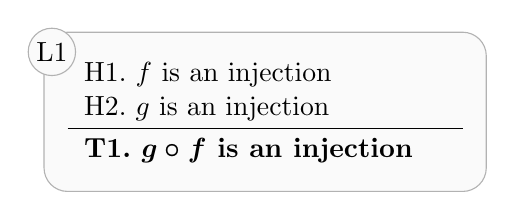
\begin{tikzpicture}[baseline=(main.base)]%
\node[tableau] (main) {%
\\

\begin{tabular}{ll}%
H1.\ $\textrm{$f$ is an injection}$&\\
H2.\ $\textrm{$g$ is an injection}$&
\Bstrut\\\hline\Tstrut
\textbf{\boldmath T1.\ $\textrm{$g\circ f$ is an injection}$\unboldmath }&\textbf{\boldmath \unboldmath }
\end{tabular}%
};%
\node[tableaulabel] at (main.north west) [xshift=4mm, yshift=-5.5mm] {L1};
\end{tikzpicture}%
\end{fit}
\smallskip

\noindent1. Expand pre-universal target T1.\nopagebreak[4] 
\marginpar{}\nopagebreak[4] 
\smallskip\nopagebreak[4] 

\begin{fit}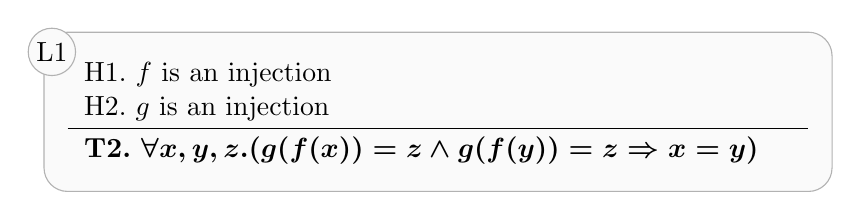
\begin{tikzpicture}[baseline=(main.base)]%
\node[tableau] (main) {%
\\

\begin{tabular}{ll}%
H1.\ $\textrm{$f$ is an injection}$&\\
H2.\ $\textrm{$g$ is an injection}$&
\Bstrut\\\hline\Tstrut
\textbf{\boldmath T2.\ $\forall x, y, z.(\textrm{$g(f(x)) = z$}\wedge \textrm{$g(f(y)) = z$}\Rightarrow \textrm{$x = y$})$\unboldmath }&\textbf{\boldmath \unboldmath }
\end{tabular}%
};%
\node[tableaulabel] at (main.north west) [xshift=4mm, yshift=-5.5mm] {L1};
\end{tikzpicture}%
\end{fit}
\smallskip

\noindent2. Apply `let' trick and move premise of universal-conditional target T2 above the line.\nopagebreak[4] 
\marginpar{Let $x$, $y$ and $z$ be such that $g(f(x)) = z$ and $g(f(y)) = z$.}\nopagebreak[4] 
\smallskip\nopagebreak[4] 

\begin{fit}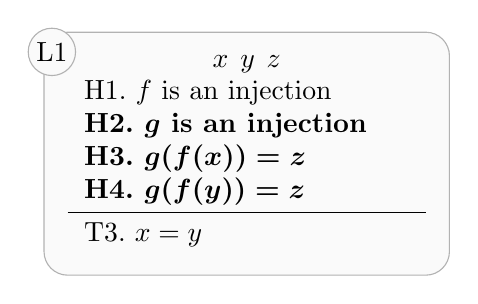
\begin{tikzpicture}[baseline=(main.base)]%
\node[tableau] (main) {%
$x$\hspace{1.5mm}$y$\hspace{1.5mm}$z$\\

\begin{tabular}{ll}%
H1.\ $\textrm{$f$ is an injection}$&\\
\textbf{\boldmath H2.\ $\textrm{$g$ is an injection}$\unboldmath }&\textbf{\boldmath \unboldmath }\\
\textbf{\boldmath H3.\ $\textrm{$g(f(x)) = z$}$\unboldmath }&\textbf{\boldmath \unboldmath }\\
\textbf{\boldmath H4.\ $\textrm{$g(f(y)) = z$}$\unboldmath }&\textbf{\boldmath \unboldmath }
\Bstrut\\\hline\Tstrut
T3.\ $\textrm{$x = y$}$&
\end{tabular}%
};%
\node[tableaulabel] at (main.north west) [xshift=4mm, yshift=-5.5mm] {L1};
\end{tikzpicture}%
\end{fit}
\smallskip

\noindent3. Forwards reasoning using H2 with (H3,H4).\nopagebreak[4] 
\marginpar{Since $g$ is an injection, $g(f(x)) = z$ and $g(f(y)) = z$, we have that $f(x) = f(y)$.}\nopagebreak[4] 
\smallskip\nopagebreak[4] 

\begin{fit}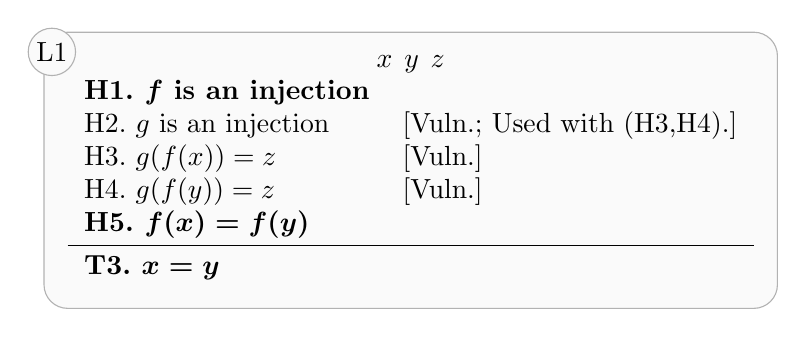
\begin{tikzpicture}[baseline=(main.base)]%
\node[tableau] (main) {%
$x$\hspace{1.5mm}$y$\hspace{1.5mm}$z$\\

\begin{tabular}{ll}%
\textbf{\boldmath H1.\ $\textrm{$f$ is an injection}$\unboldmath }&\textbf{\boldmath \unboldmath }\\
H2.\ $\textrm{$g$ is an injection}$&[Vuln.; Used with (H3,H4).]\\
H3.\ $\textrm{$g(f(x)) = z$}$&[Vuln.]\\
H4.\ $\textrm{$g(f(y)) = z$}$&[Vuln.]\\
\textbf{\boldmath H5.\ $\textrm{$f(x) = f(y)$}$\unboldmath }&\textbf{\boldmath \unboldmath }
\Bstrut\\\hline\Tstrut
\textbf{\boldmath T3.\ $\textrm{$x = y$}$\unboldmath }&\textbf{\boldmath \unboldmath }
\end{tabular}%
};%
\node[tableaulabel] at (main.north west) [xshift=4mm, yshift=-5.5mm] {L1};
\end{tikzpicture}%
\end{fit}
\smallskip

\noindent4. Backwards reasoning using H1 with (T3,H5).\nopagebreak[4] 
\marginpar{Since $f$ is an injection and $f(x) = f(y)$, $x = y$ if $f(y) = f(y)$.}\nopagebreak[4] 
\smallskip\nopagebreak[4] 

\begin{fit}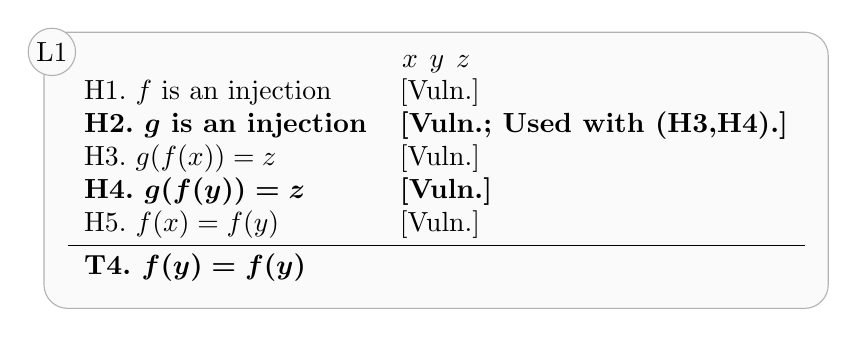
\begin{tikzpicture}[baseline=(main.base)]%
\node[tableau] (main) {%
$x$\hspace{1.5mm}$y$\hspace{1.5mm}$z$\\

\begin{tabular}{ll}%
H1.\ $\textrm{$f$ is an injection}$&[Vuln.]\\
\textbf{\boldmath H2.\ $\textrm{$g$ is an injection}$\unboldmath }&\textbf{\boldmath [Vuln.; Used with (H3,H4).]\unboldmath }\\
H3.\ $\textrm{$g(f(x)) = z$}$&[Vuln.]\\
\textbf{\boldmath H4.\ $\textrm{$g(f(y)) = z$}$\unboldmath }&\textbf{\boldmath [Vuln.]\unboldmath }\\
H5.\ $\textrm{$f(x) = f(y)$}$&[Vuln.]
\Bstrut\\\hline\Tstrut
\textbf{\boldmath T4.\ $\textrm{$f(y) = f(y)$}$\unboldmath }&\textbf{\boldmath \unboldmath }
\end{tabular}%
};%
\node[tableaulabel] at (main.north west) [xshift=4mm, yshift=-5.5mm] {L1};
\end{tikzpicture}%
\end{fit}
\smallskip

\noindent5. Backwards reasoning using H2 with (T4,H4).\nopagebreak[4] 
\marginpar{Since $g$ is an injection and $g(f(y)) = z$, $f(y) = f(y)$ if $g(f(y)) = z$.}\nopagebreak[4] 
\smallskip\nopagebreak[4] 

\begin{fit}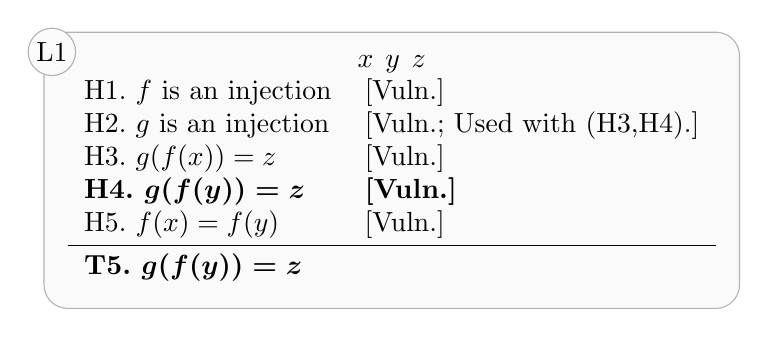
\begin{tikzpicture}[baseline=(main.base)]%
\node[tableau] (main) {%
$x$\hspace{1.5mm}$y$\hspace{1.5mm}$z$\\

\begin{tabular}{ll}%
H1.\ $\textrm{$f$ is an injection}$&[Vuln.]\\
H2.\ $\textrm{$g$ is an injection}$&[Vuln.; Used with (H3,H4).]\\
H3.\ $\textrm{$g(f(x)) = z$}$&[Vuln.]\\
\textbf{\boldmath H4.\ $\textrm{$g(f(y)) = z$}$\unboldmath }&\textbf{\boldmath [Vuln.]\unboldmath }\\
H5.\ $\textrm{$f(x) = f(y)$}$&[Vuln.]
\Bstrut\\\hline\Tstrut
\textbf{\boldmath T5.\ $\textrm{$g(f(y)) = z$}$\unboldmath }&\textbf{\boldmath \unboldmath }
\end{tabular}%
};%
\node[tableaulabel] at (main.north west) [xshift=4mm, yshift=-5.5mm] {L1};
\end{tikzpicture}%
\end{fit}
\smallskip

\noindent6. Hypothesis H4 matches target T5, so L1 is done.\nopagebreak[4] 
\marginpar{But this is clearly the case, so we are done.}\nopagebreak[4] 
\smallskip\nopagebreak[4] 

\begin{fit}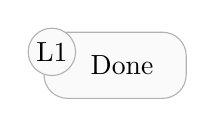
\begin{tikzpicture}%
\node[tableau] (main) {%
\ \ \,Done
};%
\node[tableaulabel] at (main.north west) [xshift=4mm, yshift=-5.5mm] {L1};
\end{tikzpicture}%
\end{fit}

Problem solved.
\cleardoublepage

\end{steps}
{\begin{center} \large \textbf{Prove that $f(A \cap B) \subset f(A) \cap f(B)$}\end{center}}\nopagebreak[4]

\begin{center}
\begin{minipage}{120mm}
By definition, since $y\in f(A\cap B)$, there exists $z\in A\cap B$ such that $f(z) = y$. Since $z\in A\cap B$, $z\in A$ and $z\in B$. We would like to show that $y\in f(A)\cap f(B)$, i.e. that $y\in f(A)$ and $y\in f(B)$. We would like to show that $y\in f(A)$. But this is clearly the case, so we are done. Thus $y\in f(B)$ and we are done.
\end{minipage}
\end{center}

\bigskip
\begin{steps}
\begin{fit}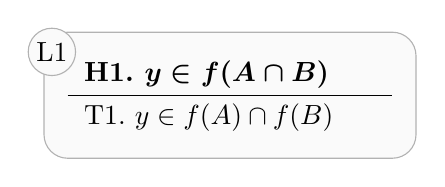
\begin{tikzpicture}[baseline=(main.base)]%
\node[tableau] (main) {%
\\

\begin{tabular}{ll}%
\textbf{\boldmath H1.\ $\textrm{$y\in f(A\cap B)$}$\unboldmath }&\textbf{\boldmath \unboldmath }
\Bstrut\\\hline\Tstrut
T1.\ $\textrm{$y\in f(A)\cap f(B)$}$&
\end{tabular}%
};%
\node[tableaulabel] at (main.north west) [xshift=4mm, yshift=-5.5mm] {L1};
\end{tikzpicture}%
\end{fit}
\smallskip

\noindent1. Expand pre-existential hypothesis H1.\nopagebreak[4] 
\marginpar{By definition, since $y\in f(A\cap B)$, there exists $z\in A\cap B$ such that $f(z) = y$.}\nopagebreak[4] 
\smallskip\nopagebreak[4] 

\begin{fit}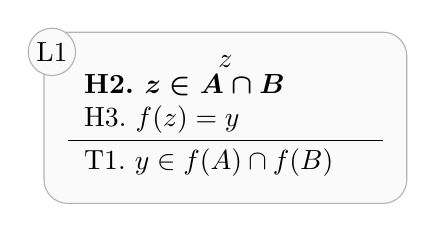
\begin{tikzpicture}[baseline=(main.base)]%
\node[tableau] (main) {%
$z$\\

\begin{tabular}{ll}%
\textbf{\boldmath H2.\ $\textrm{$z\in A\cap B$}$\unboldmath }&\textbf{\boldmath \unboldmath }\\
H3.\ $\textrm{$f(z) = y$}$&
\Bstrut\\\hline\Tstrut
T1.\ $\textrm{$y\in f(A)\cap f(B)$}$&
\end{tabular}%
};%
\node[tableaulabel] at (main.north west) [xshift=4mm, yshift=-5.5mm] {L1};
\end{tikzpicture}%
\end{fit}
\smallskip

\noindent2. Quantifier-free expansion of hypothesis H2.\nopagebreak[4] 
\marginpar{Since $z\in A\cap B$, $z\in A$ and $z\in B$.}\nopagebreak[4] 
\smallskip\nopagebreak[4] 

\begin{fit}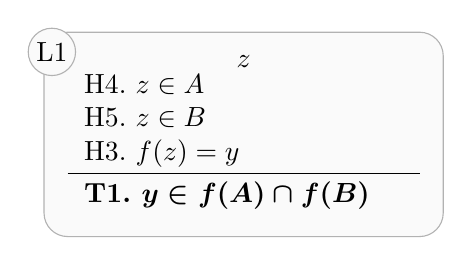
\begin{tikzpicture}[baseline=(main.base)]%
\node[tableau] (main) {%
$z$\\

\begin{tabular}{ll}%
H4.\ $\textrm{$z\in A$}$&\\
H5.\ $\textrm{$z\in B$}$&\\
H3.\ $\textrm{$f(z) = y$}$&
\Bstrut\\\hline\Tstrut
\textbf{\boldmath T1.\ $\textrm{$y\in f(A)\cap f(B)$}$\unboldmath }&\textbf{\boldmath \unboldmath }
\end{tabular}%
};%
\node[tableaulabel] at (main.north west) [xshift=4mm, yshift=-5.5mm] {L1};
\end{tikzpicture}%
\end{fit}
\smallskip

\noindent3. Quantifier-free expansion of target T1.\nopagebreak[4] 
\marginpar{We would like to show that $y\in f(A)\cap f(B)$, i.e. that $y\in f(A)$ and $y\in f(B)$.}\nopagebreak[4] 
\smallskip\nopagebreak[4] 

\begin{fit}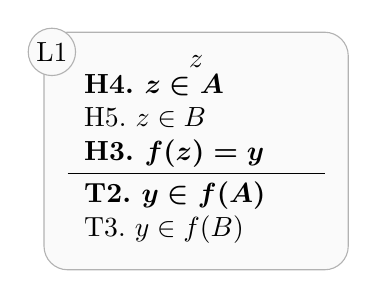
\begin{tikzpicture}[baseline=(main.base)]%
\node[tableau] (main) {%
$z$\\

\begin{tabular}{ll}%
\textbf{\boldmath H4.\ $\textrm{$z\in A$}$\unboldmath }&\textbf{\boldmath \unboldmath }\\
H5.\ $\textrm{$z\in B$}$&\\
\textbf{\boldmath H3.\ $\textrm{$f(z) = y$}$\unboldmath }&\textbf{\boldmath \unboldmath }
\Bstrut\\\hline\Tstrut
\textbf{\boldmath T2.\ $\textrm{$y\in f(A)$}$\unboldmath }&\textbf{\boldmath \unboldmath }\\
T3.\ $\textrm{$y\in f(B)$}$&
\end{tabular}%
};%
\node[tableaulabel] at (main.north west) [xshift=4mm, yshift=-5.5mm] {L1};
\end{tikzpicture}%
\end{fit}
\smallskip

\noindent4. All conjuncts of T2 (after expansion) can be simultaneously matched against H4 and H3 or rendered trivial by choosing $u = z$, so we can remove T2.\nopagebreak[4] 
\marginpar{We would like to show that $y\in f(A)$. But this is clearly the case, so we are done.}\nopagebreak[4] 
\smallskip\nopagebreak[4] 

\begin{fit}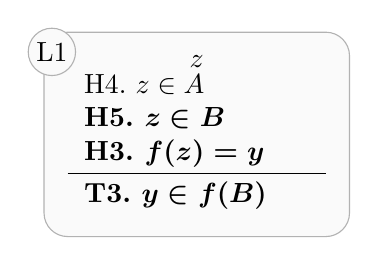
\begin{tikzpicture}[baseline=(main.base)]%
\node[tableau] (main) {%
$z$\\

\begin{tabular}{ll}%
H4.\ $\textrm{$z\in A$}$&\\
\textbf{\boldmath H5.\ $\textrm{$z\in B$}$\unboldmath }&\textbf{\boldmath \unboldmath }\\
\textbf{\boldmath H3.\ $\textrm{$f(z) = y$}$\unboldmath }&\textbf{\boldmath \unboldmath }
\Bstrut\\\hline\Tstrut
\textbf{\boldmath T3.\ $\textrm{$y\in f(B)$}$\unboldmath }&\textbf{\boldmath \unboldmath }
\end{tabular}%
};%
\node[tableaulabel] at (main.north west) [xshift=4mm, yshift=-5.5mm] {L1};
\end{tikzpicture}%
\end{fit}
\smallskip

\noindent5. All conjuncts of T3 (after expansion) can be simultaneously matched against H5 and H3 or rendered trivial by choosing $u = z$, so L1 is done.\nopagebreak[4] 
\marginpar{We would like to show that $y\in f(B)$. But this is clearly the case, so we are done.}\nopagebreak[4] 
\smallskip\nopagebreak[4] 

\begin{fit}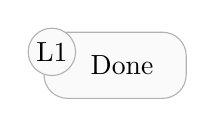
\begin{tikzpicture}%
\node[tableau] (main) {%
\ \ \,Done
};%
\node[tableaulabel] at (main.north west) [xshift=4mm, yshift=-5.5mm] {L1};
\end{tikzpicture}%
\end{fit}

Problem solved.
\cleardoublepage

\end{steps}
{\begin{center} \large \textbf{Prove that $f^{-1}(A \cap B) \subset f^{-1}(A) \cap f^{-1}(B)$}\end{center}}\nopagebreak[4]

\begin{center}
\begin{minipage}{120mm}
Since $x\in f^{-1}(A\cap B)$, we have that $f(x)\in A\cap B$. Then $f(x)\in A$ and $f(x)\in B$. We would like to show that $x\in f^{-1}(A)\cap f^{-1}(B)$, i.e. that $x\in f^{-1}(A)$ and $x\in f^{-1}(B)$. We would like to show that $x\in f^{-1}(A)$, i.e. that $f(x)\in A$. We would like to show that $x\in f^{-1}(B)$, i.e. that $f(x)\in B$. But this is clearly the case, so we are done.
\end{minipage}
\end{center}

\bigskip
\begin{steps}
\begin{fit}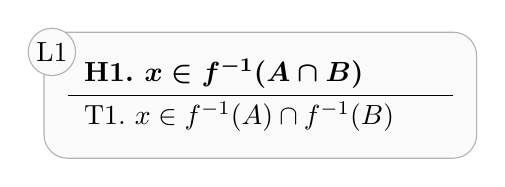
\begin{tikzpicture}[baseline=(main.base)]%
\node[tableau] (main) {%
\\

\begin{tabular}{ll}%
\textbf{\boldmath H1.\ $\textrm{$x\in f^{-1}(A\cap B)$}$\unboldmath }&\textbf{\boldmath \unboldmath }
\Bstrut\\\hline\Tstrut
T1.\ $\textrm{$x\in f^{-1}(A)\cap f^{-1}(B)$}$&
\end{tabular}%
};%
\node[tableaulabel] at (main.north west) [xshift=4mm, yshift=-5.5mm] {L1};
\end{tikzpicture}%
\end{fit}
\smallskip

\noindent1. Quantifier-free expansion of hypothesis H1.\nopagebreak[4] 
\marginpar{Since $x\in f^{-1}(A\cap B)$, we have that $f(x)\in A\cap B$.}\nopagebreak[4] 
\smallskip\nopagebreak[4] 

\begin{fit}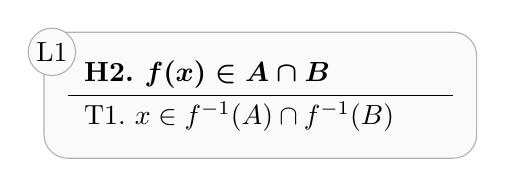
\begin{tikzpicture}[baseline=(main.base)]%
\node[tableau] (main) {%
\\

\begin{tabular}{ll}%
\textbf{\boldmath H2.\ $\textrm{$f(x)\in A\cap B$}$\unboldmath }&\textbf{\boldmath \unboldmath }
\Bstrut\\\hline\Tstrut
T1.\ $\textrm{$x\in f^{-1}(A)\cap f^{-1}(B)$}$&
\end{tabular}%
};%
\node[tableaulabel] at (main.north west) [xshift=4mm, yshift=-5.5mm] {L1};
\end{tikzpicture}%
\end{fit}
\smallskip

\noindent2. Quantifier-free expansion of hypothesis H2.\nopagebreak[4] 
\marginpar{Since $f(x)\in A\cap B$, $f(x)\in A$ and $f(x)\in B$.}\nopagebreak[4] 
\smallskip\nopagebreak[4] 

\begin{fit}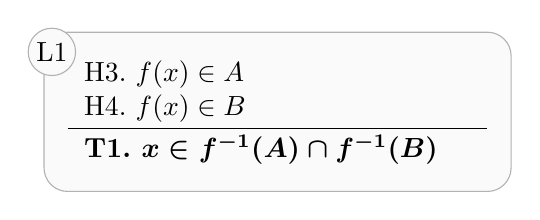
\begin{tikzpicture}[baseline=(main.base)]%
\node[tableau] (main) {%
\\

\begin{tabular}{ll}%
H3.\ $\textrm{$f(x)\in A$}$&\\
H4.\ $\textrm{$f(x)\in B$}$&
\Bstrut\\\hline\Tstrut
\textbf{\boldmath T1.\ $\textrm{$x\in f^{-1}(A)\cap f^{-1}(B)$}$\unboldmath }&\textbf{\boldmath \unboldmath }
\end{tabular}%
};%
\node[tableaulabel] at (main.north west) [xshift=4mm, yshift=-5.5mm] {L1};
\end{tikzpicture}%
\end{fit}
\smallskip

\noindent3. Quantifier-free expansion of target T1.\nopagebreak[4] 
\marginpar{We would like to show that $x\in f^{-1}(A)\cap f^{-1}(B)$, i.e. that $x\in f^{-1}(A)$ and $x\in f^{-1}(B)$.}\nopagebreak[4] 
\smallskip\nopagebreak[4] 

\begin{fit}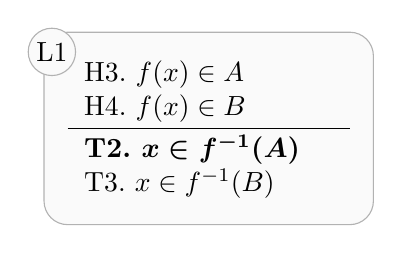
\begin{tikzpicture}[baseline=(main.base)]%
\node[tableau] (main) {%
\\

\begin{tabular}{ll}%
H3.\ $\textrm{$f(x)\in A$}$&\\
H4.\ $\textrm{$f(x)\in B$}$&
\Bstrut\\\hline\Tstrut
\textbf{\boldmath T2.\ $\textrm{$x\in f^{-1}(A)$}$\unboldmath }&\textbf{\boldmath \unboldmath }\\
T3.\ $\textrm{$x\in f^{-1}(B)$}$&
\end{tabular}%
};%
\node[tableaulabel] at (main.north west) [xshift=4mm, yshift=-5.5mm] {L1};
\end{tikzpicture}%
\end{fit}
\smallskip

\noindent4. Quantifier-free expansion of target T2.\nopagebreak[4] 
\marginpar{We would like to show that $x\in f^{-1}(A)$, i.e. that $f(x)\in A$.}\nopagebreak[4] 
\smallskip\nopagebreak[4] 

\begin{fit}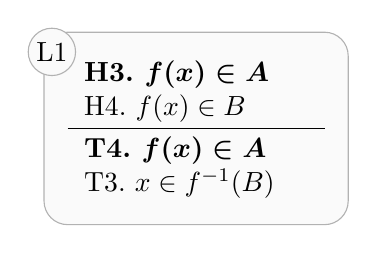
\begin{tikzpicture}[baseline=(main.base)]%
\node[tableau] (main) {%
\\

\begin{tabular}{ll}%
\textbf{\boldmath H3.\ $\textrm{$f(x)\in A$}$\unboldmath }&\textbf{\boldmath \unboldmath }\\
H4.\ $\textrm{$f(x)\in B$}$&
\Bstrut\\\hline\Tstrut
\textbf{\boldmath T4.\ $\textrm{$f(x)\in A$}$\unboldmath }&\textbf{\boldmath \unboldmath }\\
T3.\ $\textrm{$x\in f^{-1}(B)$}$&
\end{tabular}%
};%
\node[tableaulabel] at (main.north west) [xshift=4mm, yshift=-5.5mm] {L1};
\end{tikzpicture}%
\end{fit}
\smallskip

\noindent5. Hypothesis H3 matches target T4, so we can remove T4.\nopagebreak[4] 
\marginpar{}\nopagebreak[4] 
\smallskip\nopagebreak[4] 

\begin{fit}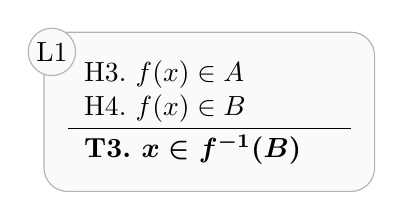
\begin{tikzpicture}[baseline=(main.base)]%
\node[tableau] (main) {%
\\

\begin{tabular}{ll}%
H3.\ $\textrm{$f(x)\in A$}$&\\
H4.\ $\textrm{$f(x)\in B$}$&
\Bstrut\\\hline\Tstrut
\textbf{\boldmath T3.\ $\textrm{$x\in f^{-1}(B)$}$\unboldmath }&\textbf{\boldmath \unboldmath }
\end{tabular}%
};%
\node[tableaulabel] at (main.north west) [xshift=4mm, yshift=-5.5mm] {L1};
\end{tikzpicture}%
\end{fit}
\smallskip

\noindent6. Quantifier-free expansion of target T3.\nopagebreak[4] 
\marginpar{We would like to show that $x\in f^{-1}(B)$, i.e. that $f(x)\in B$.}\nopagebreak[4] 
\smallskip\nopagebreak[4] 

\begin{fit}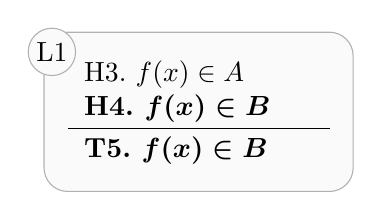
\begin{tikzpicture}[baseline=(main.base)]%
\node[tableau] (main) {%
\\

\begin{tabular}{ll}%
H3.\ $\textrm{$f(x)\in A$}$&\\
\textbf{\boldmath H4.\ $\textrm{$f(x)\in B$}$\unboldmath }&\textbf{\boldmath \unboldmath }
\Bstrut\\\hline\Tstrut
\textbf{\boldmath T5.\ $\textrm{$f(x)\in B$}$\unboldmath }&\textbf{\boldmath \unboldmath }
\end{tabular}%
};%
\node[tableaulabel] at (main.north west) [xshift=4mm, yshift=-5.5mm] {L1};
\end{tikzpicture}%
\end{fit}
\smallskip

\noindent7. Hypothesis H4 matches target T5, so L1 is done.\nopagebreak[4] 
\marginpar{But this is clearly the case, so we are done.}\nopagebreak[4] 
\smallskip\nopagebreak[4] 

\begin{fit}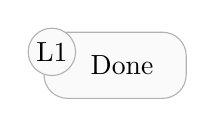
\begin{tikzpicture}%
\node[tableau] (main) {%
\ \ \,Done
};%
\node[tableaulabel] at (main.north west) [xshift=4mm, yshift=-5.5mm] {L1};
\end{tikzpicture}%
\end{fit}

Problem solved.
\cleardoublepage

\end{steps}
{\begin{center} \large \textbf{Prove that $f^{-1}(A) \cap f^{-1}(B) \subset f^{-1}(A \cap B)$}\end{center}}\nopagebreak[4]

\begin{center}
\begin{minipage}{120mm}
Let $x$ be an element of $f^{-1}(A)\cap f^{-1}(B)$. Then $x\in f^{-1}(A)$ and $x\in f^{-1}(B)$. Then $f(x)\in A$ and $f(x)\in B$. We would like to show that $x\in f^{-1}(A\cap B)$, i.e. that $f(x)\in A\cap B$. We would like to show that $f(x)\in A\cap B$, i.e. that $f(x)\in A$ and $f(x)\in B$. But this is clearly the case, so we are done.
\end{minipage}
\end{center}

\bigskip
\begin{steps}
\begin{fit}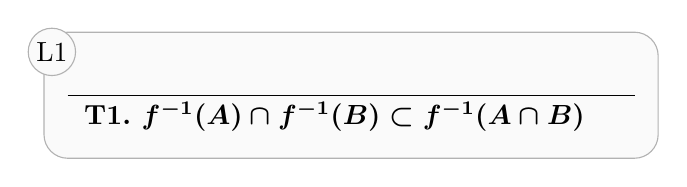
\begin{tikzpicture}[baseline=(main.base)]%
\node[tableau] (main) {%
\\

\begin{tabular}{ll}%

\Bstrut\\\hline\Tstrut
\textbf{\boldmath T1.\ $\textrm{$f^{-1}(A)\cap f^{-1}(B)\subset f^{-1}(A\cap B)$}$\unboldmath }&\textbf{\boldmath \unboldmath }
\end{tabular}%
};%
\node[tableaulabel] at (main.north west) [xshift=4mm, yshift=-5.5mm] {L1};
\end{tikzpicture}%
\end{fit}
\smallskip

\noindent1. Expand pre-universal target T1.\nopagebreak[4] 
\marginpar{}\nopagebreak[4] 
\smallskip\nopagebreak[4] 

\begin{fit}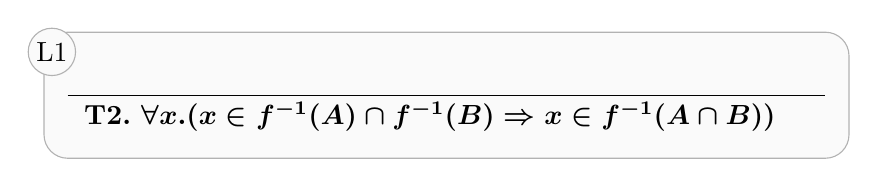
\begin{tikzpicture}[baseline=(main.base)]%
\node[tableau] (main) {%
\\

\begin{tabular}{ll}%

\Bstrut\\\hline\Tstrut
\textbf{\boldmath T2.\ $\forall x.(\textrm{$x\in f^{-1}(A)\cap f^{-1}(B)$}\Rightarrow \textrm{$x\in f^{-1}(A\cap B)$})$\unboldmath }&\textbf{\boldmath \unboldmath }
\end{tabular}%
};%
\node[tableaulabel] at (main.north west) [xshift=4mm, yshift=-5.5mm] {L1};
\end{tikzpicture}%
\end{fit}
\smallskip

\noindent2. Apply `let' trick and move premise of universal-conditional target T2 above the line.\nopagebreak[4] 
\marginpar{Let $x$ be an element of $f^{-1}(A)\cap f^{-1}(B)$.}\nopagebreak[4] 
\smallskip\nopagebreak[4] 

\begin{fit}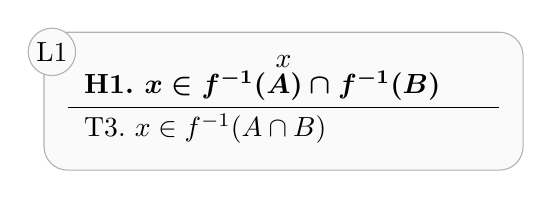
\begin{tikzpicture}[baseline=(main.base)]%
\node[tableau] (main) {%
$x$\\

\begin{tabular}{ll}%
\textbf{\boldmath H1.\ $\textrm{$x\in f^{-1}(A)\cap f^{-1}(B)$}$\unboldmath }&\textbf{\boldmath \unboldmath }
\Bstrut\\\hline\Tstrut
T3.\ $\textrm{$x\in f^{-1}(A\cap B)$}$&
\end{tabular}%
};%
\node[tableaulabel] at (main.north west) [xshift=4mm, yshift=-5.5mm] {L1};
\end{tikzpicture}%
\end{fit}
\smallskip

\noindent3. Quantifier-free expansion of hypothesis H1.\nopagebreak[4] 
\marginpar{Since $x\in f^{-1}(A)\cap f^{-1}(B)$, $x\in f^{-1}(A)$ and $x\in f^{-1}(B)$.}\nopagebreak[4] 
\smallskip\nopagebreak[4] 

\begin{fit}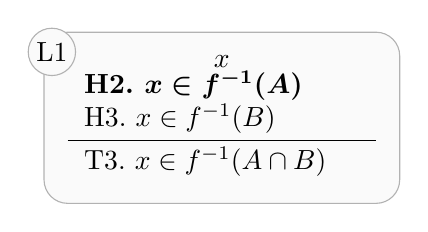
\begin{tikzpicture}[baseline=(main.base)]%
\node[tableau] (main) {%
$x$\\

\begin{tabular}{ll}%
\textbf{\boldmath H2.\ $\textrm{$x\in f^{-1}(A)$}$\unboldmath }&\textbf{\boldmath \unboldmath }\\
H3.\ $\textrm{$x\in f^{-1}(B)$}$&
\Bstrut\\\hline\Tstrut
T3.\ $\textrm{$x\in f^{-1}(A\cap B)$}$&
\end{tabular}%
};%
\node[tableaulabel] at (main.north west) [xshift=4mm, yshift=-5.5mm] {L1};
\end{tikzpicture}%
\end{fit}
\smallskip

\noindent4. Quantifier-free expansion of hypothesis H2.\nopagebreak[4] 
\marginpar{Since $x\in f^{-1}(A)$, we have that $f(x)\in A$.}\nopagebreak[4] 
\smallskip\nopagebreak[4] 

\begin{fit}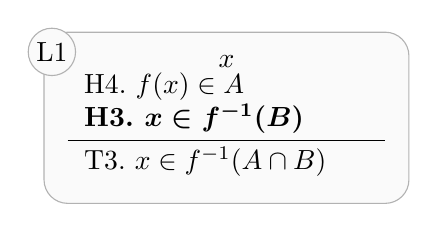
\begin{tikzpicture}[baseline=(main.base)]%
\node[tableau] (main) {%
$x$\\

\begin{tabular}{ll}%
H4.\ $\textrm{$f(x)\in A$}$&\\
\textbf{\boldmath H3.\ $\textrm{$x\in f^{-1}(B)$}$\unboldmath }&\textbf{\boldmath \unboldmath }
\Bstrut\\\hline\Tstrut
T3.\ $\textrm{$x\in f^{-1}(A\cap B)$}$&
\end{tabular}%
};%
\node[tableaulabel] at (main.north west) [xshift=4mm, yshift=-5.5mm] {L1};
\end{tikzpicture}%
\end{fit}
\smallskip

\noindent5. Quantifier-free expansion of hypothesis H3.\nopagebreak[4] 
\marginpar{Since $x\in f^{-1}(B)$, we have that $f(x)\in B$.}\nopagebreak[4] 
\smallskip\nopagebreak[4] 

\begin{fit}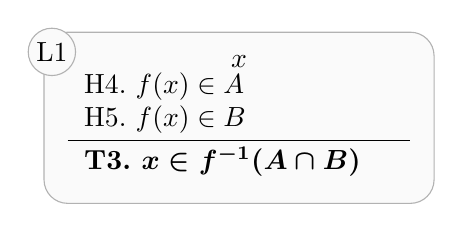
\begin{tikzpicture}[baseline=(main.base)]%
\node[tableau] (main) {%
$x$\\

\begin{tabular}{ll}%
H4.\ $\textrm{$f(x)\in A$}$&\\
H5.\ $\textrm{$f(x)\in B$}$&
\Bstrut\\\hline\Tstrut
\textbf{\boldmath T3.\ $\textrm{$x\in f^{-1}(A\cap B)$}$\unboldmath }&\textbf{\boldmath \unboldmath }
\end{tabular}%
};%
\node[tableaulabel] at (main.north west) [xshift=4mm, yshift=-5.5mm] {L1};
\end{tikzpicture}%
\end{fit}
\smallskip

\noindent6. Quantifier-free expansion of target T3.\nopagebreak[4] 
\marginpar{We would like to show that $x\in f^{-1}(A\cap B)$, i.e. that $f(x)\in A\cap B$.}\nopagebreak[4] 
\smallskip\nopagebreak[4] 

\begin{fit}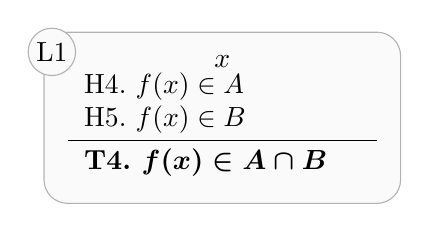
\begin{tikzpicture}[baseline=(main.base)]%
\node[tableau] (main) {%
$x$\\

\begin{tabular}{ll}%
H4.\ $\textrm{$f(x)\in A$}$&\\
H5.\ $\textrm{$f(x)\in B$}$&
\Bstrut\\\hline\Tstrut
\textbf{\boldmath T4.\ $\textrm{$f(x)\in A\cap B$}$\unboldmath }&\textbf{\boldmath \unboldmath }
\end{tabular}%
};%
\node[tableaulabel] at (main.north west) [xshift=4mm, yshift=-5.5mm] {L1};
\end{tikzpicture}%
\end{fit}
\smallskip

\noindent7. Quantifier-free expansion of target T4.\nopagebreak[4] 
\marginpar{We would like to show that $f(x)\in A\cap B$, i.e. that $f(x)\in A$ and $f(x)\in B$.}\nopagebreak[4] 
\smallskip\nopagebreak[4] 

\begin{fit}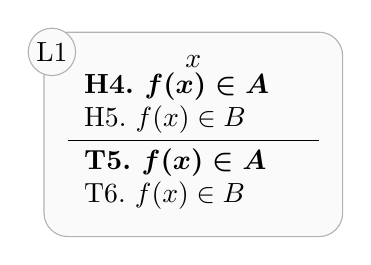
\begin{tikzpicture}[baseline=(main.base)]%
\node[tableau] (main) {%
$x$\\

\begin{tabular}{ll}%
\textbf{\boldmath H4.\ $\textrm{$f(x)\in A$}$\unboldmath }&\textbf{\boldmath \unboldmath }\\
H5.\ $\textrm{$f(x)\in B$}$&
\Bstrut\\\hline\Tstrut
\textbf{\boldmath T5.\ $\textrm{$f(x)\in A$}$\unboldmath }&\textbf{\boldmath \unboldmath }\\
T6.\ $\textrm{$f(x)\in B$}$&
\end{tabular}%
};%
\node[tableaulabel] at (main.north west) [xshift=4mm, yshift=-5.5mm] {L1};
\end{tikzpicture}%
\end{fit}
\smallskip

\noindent8. Hypothesis H4 matches target T5, so we can remove T5.\nopagebreak[4] 
\marginpar{}\nopagebreak[4] 
\smallskip\nopagebreak[4] 

\begin{fit}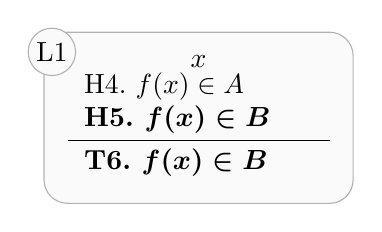
\begin{tikzpicture}[baseline=(main.base)]%
\node[tableau] (main) {%
$x$\\

\begin{tabular}{ll}%
H4.\ $\textrm{$f(x)\in A$}$&\\
\textbf{\boldmath H5.\ $\textrm{$f(x)\in B$}$\unboldmath }&\textbf{\boldmath \unboldmath }
\Bstrut\\\hline\Tstrut
\textbf{\boldmath T6.\ $\textrm{$f(x)\in B$}$\unboldmath }&\textbf{\boldmath \unboldmath }
\end{tabular}%
};%
\node[tableaulabel] at (main.north west) [xshift=4mm, yshift=-5.5mm] {L1};
\end{tikzpicture}%
\end{fit}
\smallskip

\noindent9. Hypothesis H5 matches target T6, so L1 is done.\nopagebreak[4] 
\marginpar{But this is clearly the case, so we are done.}\nopagebreak[4] 
\smallskip\nopagebreak[4] 

\begin{fit}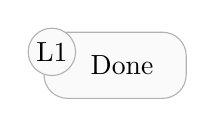
\begin{tikzpicture}%
\node[tableau] (main) {%
\ \ \,Done
};%
\node[tableaulabel] at (main.north west) [xshift=4mm, yshift=-5.5mm] {L1};
\end{tikzpicture}%
\end{fit}

Problem solved.
\cleardoublepage

\end{steps}
{\begin{center} \large \textbf{Prove that $f^{-1}(A \cup B) \subset f^{-1}(A) \cup f^{-1}(B)$}\end{center}}\nopagebreak[4]

\begin{center}
\begin{minipage}{120mm}
Let $x$ be an element of $f^{-1}(A\cup B)$. Then $f(x)\in A\cup B$. Then $f(x)\in A$ or $f(x)\in B$. We would like to show that $x\in f^{-1}(A)\cup f^{-1}(B)$, i.e. that $x\in f^{-1}(A)$ or $x\in f^{-1}(B)$. We would like to show that $x\in f^{-1}(A)$, i.e. that $f(x)\in A$. But this is clearly the case, so we are done. We would like to show that $x\in f^{-1}(A)\cup f^{-1}(B)$, i.e. that $x\in f^{-1}(A)$ or $x\in f^{-1}(B)$. We would like to show that $x\in f^{-1}(A)$, i.e. that $f(x)\in A$. We would like to show that $x\in f^{-1}(B)$, i.e. that $f(x)\in B$. But this is clearly the case, so we are done.
\end{minipage}
\end{center}

\bigskip
\begin{steps}
\begin{fit}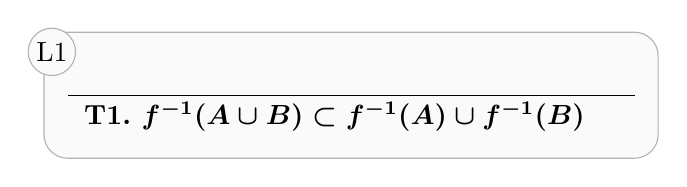
\begin{tikzpicture}[baseline=(main.base)]%
\node[tableau] (main) {%
\\

\begin{tabular}{ll}%

\Bstrut\\\hline\Tstrut
\textbf{\boldmath T1.\ $\textrm{$f^{-1}(A\cup B)\subset f^{-1}(A)\cup f^{-1}(B)$}$\unboldmath }&\textbf{\boldmath \unboldmath }
\end{tabular}%
};%
\node[tableaulabel] at (main.north west) [xshift=4mm, yshift=-5.5mm] {L1};
\end{tikzpicture}%
\end{fit}
\smallskip

\noindent1. Expand pre-universal target T1.\nopagebreak[4] 
\marginpar{}\nopagebreak[4] 
\smallskip\nopagebreak[4] 

\begin{fit}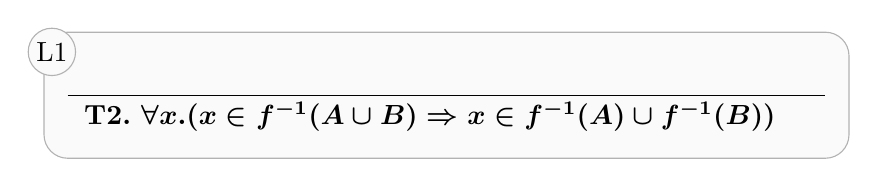
\begin{tikzpicture}[baseline=(main.base)]%
\node[tableau] (main) {%
\\

\begin{tabular}{ll}%

\Bstrut\\\hline\Tstrut
\textbf{\boldmath T2.\ $\forall x.(\textrm{$x\in f^{-1}(A\cup B)$}\Rightarrow \textrm{$x\in f^{-1}(A)\cup f^{-1}(B)$})$\unboldmath }&\textbf{\boldmath \unboldmath }
\end{tabular}%
};%
\node[tableaulabel] at (main.north west) [xshift=4mm, yshift=-5.5mm] {L1};
\end{tikzpicture}%
\end{fit}
\smallskip

\noindent2. Apply `let' trick and move premise of universal-conditional target T2 above the line.\nopagebreak[4] 
\marginpar{Let $x$ be an element of $f^{-1}(A\cup B)$.}\nopagebreak[4] 
\smallskip\nopagebreak[4] 

\begin{fit}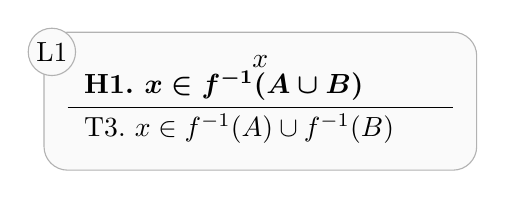
\begin{tikzpicture}[baseline=(main.base)]%
\node[tableau] (main) {%
$x$\\

\begin{tabular}{ll}%
\textbf{\boldmath H1.\ $\textrm{$x\in f^{-1}(A\cup B)$}$\unboldmath }&\textbf{\boldmath \unboldmath }
\Bstrut\\\hline\Tstrut
T3.\ $\textrm{$x\in f^{-1}(A)\cup f^{-1}(B)$}$&
\end{tabular}%
};%
\node[tableaulabel] at (main.north west) [xshift=4mm, yshift=-5.5mm] {L1};
\end{tikzpicture}%
\end{fit}
\smallskip

\noindent3. Quantifier-free expansion of hypothesis H1.\nopagebreak[4] 
\marginpar{Since $x\in f^{-1}(A\cup B)$, we have that $f(x)\in A\cup B$.}\nopagebreak[4] 
\smallskip\nopagebreak[4] 

\begin{fit}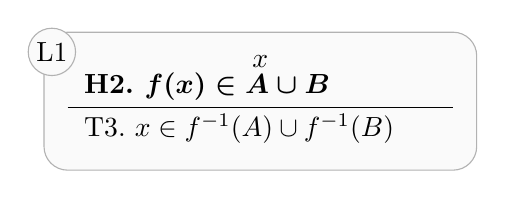
\begin{tikzpicture}[baseline=(main.base)]%
\node[tableau] (main) {%
$x$\\

\begin{tabular}{ll}%
\textbf{\boldmath H2.\ $\textrm{$f(x)\in A\cup B$}$\unboldmath }&\textbf{\boldmath \unboldmath }
\Bstrut\\\hline\Tstrut
T3.\ $\textrm{$x\in f^{-1}(A)\cup f^{-1}(B)$}$&
\end{tabular}%
};%
\node[tableaulabel] at (main.north west) [xshift=4mm, yshift=-5.5mm] {L1};
\end{tikzpicture}%
\end{fit}
\smallskip

\noindent4. Quantifier-free expansion of hypothesis H2.\nopagebreak[4] 
\marginpar{Since $f(x)\in A\cup B$, $f(x)\in A$ or $f(x)\in B$.}\nopagebreak[4] 
\smallskip\nopagebreak[4] 

\begin{fit}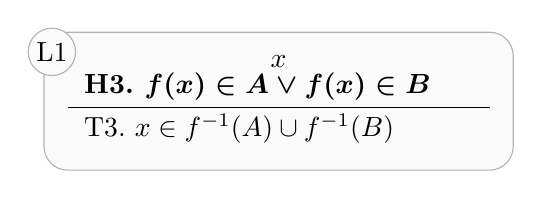
\begin{tikzpicture}[baseline=(main.base)]%
\node[tableau] (main) {%
$x$\\

\begin{tabular}{ll}%
\textbf{\boldmath H3.\ $\textrm{$f(x)\in A$}\vee \textrm{$f(x)\in B$}$\unboldmath }&\textbf{\boldmath \unboldmath }
\Bstrut\\\hline\Tstrut
T3.\ $\textrm{$x\in f^{-1}(A)\cup f^{-1}(B)$}$&
\end{tabular}%
};%
\node[tableaulabel] at (main.north west) [xshift=4mm, yshift=-5.5mm] {L1};
\end{tikzpicture}%
\end{fit}
\smallskip

\noindent5. Split into cases to handle disjunctive hypothesis H3.\nopagebreak[4] 
\marginpar{}\nopagebreak[4] 
\smallskip\nopagebreak[4] 

\begin{fit}\begin{tikzpicture}[baseline=(main.base)]%
\node[tableau] (main) {%
$x$\\

\begin{tabular}{ll}%

\Bstrut\\\hline\Tstrut
\begin{tikzpicture}[baseline=(main.base)]%
\node[tableau] (main) {%
\\

\begin{tabular}{ll}%
H4.\ $\textrm{$f(x)\in A$}$&
\Bstrut\\\hline\Tstrut
\textbf{\boldmath T4.\ $\textrm{$x\in f^{-1}(A)\cup f^{-1}(B)$}$\unboldmath }&\textbf{\boldmath \unboldmath }
\end{tabular}%
};%
\node[tableaulabel] at (main.north west) [xshift=4mm, yshift=-5.5mm] {L2};
\end{tikzpicture}%
\\
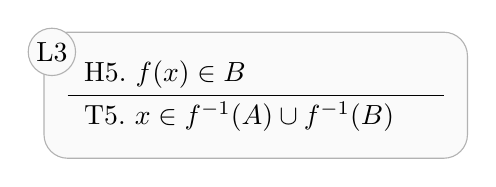
\begin{tikzpicture}[baseline=(main.base)]%
\node[tableau] (main) {%
\\

\begin{tabular}{ll}%
H5.\ $\textrm{$f(x)\in B$}$&
\Bstrut\\\hline\Tstrut
T5.\ $\textrm{$x\in f^{-1}(A)\cup f^{-1}(B)$}$&
\end{tabular}%
};%
\node[tableaulabel] at (main.north west) [xshift=4mm, yshift=-5.5mm] {L3};
\end{tikzpicture}%

\end{tabular}%
};%
\node[tableaulabel] at (main.north west) [xshift=4mm, yshift=-5.5mm] {L1};
\end{tikzpicture}%
\end{fit}
\smallskip

\noindent6. Quantifier-free expansion of target T4.\nopagebreak[4] 
\marginpar{We would like to show that $x\in f^{-1}(A)\cup f^{-1}(B)$, i.e. that $x\in f^{-1}(A)$ or $x\in f^{-1}(B)$.}\nopagebreak[4] 
\smallskip\nopagebreak[4] 

\begin{fit}\begin{tikzpicture}[baseline=(main.base)]%
\node[tableau] (main) {%
$x$\\

\begin{tabular}{ll}%

\Bstrut\\\hline\Tstrut
\begin{tikzpicture}[baseline=(main.base)]%
\node[tableau] (main) {%
\\

\begin{tabular}{ll}%
H4.\ $\textrm{$f(x)\in A$}$&
\Bstrut\\\hline\Tstrut
\textbf{\boldmath T6.\ $\textrm{$x\in f^{-1}(A)$}\vee \textrm{$x\in f^{-1}(B)$}$\unboldmath }&\textbf{\boldmath \unboldmath }
\end{tabular}%
};%
\node[tableaulabel] at (main.north west) [xshift=4mm, yshift=-5.5mm] {L2};
\end{tikzpicture}%
\\
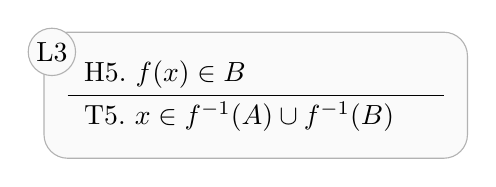
\begin{tikzpicture}[baseline=(main.base)]%
\node[tableau] (main) {%
\\

\begin{tabular}{ll}%
H5.\ $\textrm{$f(x)\in B$}$&
\Bstrut\\\hline\Tstrut
T5.\ $\textrm{$x\in f^{-1}(A)\cup f^{-1}(B)$}$&
\end{tabular}%
};%
\node[tableaulabel] at (main.north west) [xshift=4mm, yshift=-5.5mm] {L3};
\end{tikzpicture}%

\end{tabular}%
};%
\node[tableaulabel] at (main.north west) [xshift=4mm, yshift=-5.5mm] {L1};
\end{tikzpicture}%
\end{fit}
\smallskip

\noindent7. Split up disjunctive target T6.\nopagebreak[4] 
\marginpar{}\nopagebreak[4] 
\smallskip\nopagebreak[4] 

\begin{fit}\begin{tikzpicture}[baseline=(main.base)]%
\node[tableau] (main) {%
$x$\\

\begin{tabular}{ll}%

\Bstrut\\\hline\Tstrut
\begin{tikzpicture}[baseline=(main.base)]%
\node[tableau] (main) {%
\\

\begin{tabular}{ll}%
H4.\ $\textrm{$f(x)\in A$}$&
\Bstrut\\\hline\Tstrut
\begin{tikzpicture}[baseline=(main.base)]%
\node[tableau] (main) {%
\\

\begin{tabular}{ll}%

\Bstrut\\\hline\Tstrut
\textbf{\boldmath T9.\ $\textrm{$x\in f^{-1}(A)$}$\unboldmath }&\textbf{\boldmath \unboldmath }
\end{tabular}%
};%
\node[tableaulabel] at (main.north west) [xshift=4mm, yshift=-5.5mm] {L6};
\end{tikzpicture}%
\hspace{2mm}$\vee$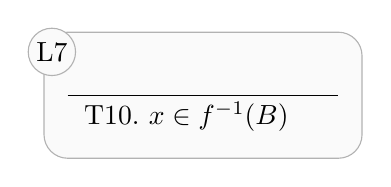
\begin{tikzpicture}[baseline=(main.base)]%
\node[tableau] (main) {%
\\

\begin{tabular}{ll}%

\Bstrut\\\hline\Tstrut
T10.\ $\textrm{$x\in f^{-1}(B)$}$&
\end{tabular}%
};%
\node[tableaulabel] at (main.north west) [xshift=4mm, yshift=-5.5mm] {L7};
\end{tikzpicture}%

\end{tabular}%
};%
\node[tableaulabel] at (main.north west) [xshift=4mm, yshift=-5.5mm] {L2};
\end{tikzpicture}%
\\
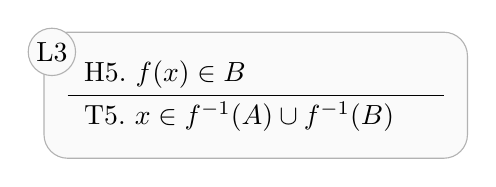
\begin{tikzpicture}[baseline=(main.base)]%
\node[tableau] (main) {%
\\

\begin{tabular}{ll}%
H5.\ $\textrm{$f(x)\in B$}$&
\Bstrut\\\hline\Tstrut
T5.\ $\textrm{$x\in f^{-1}(A)\cup f^{-1}(B)$}$&
\end{tabular}%
};%
\node[tableaulabel] at (main.north west) [xshift=4mm, yshift=-5.5mm] {L3};
\end{tikzpicture}%

\end{tabular}%
};%
\node[tableaulabel] at (main.north west) [xshift=4mm, yshift=-5.5mm] {L1};
\end{tikzpicture}%
\end{fit}
\smallskip

\noindent8. Quantifier-free expansion of target T9.\nopagebreak[4] 
\marginpar{We would like to show that $x\in f^{-1}(A)$, i.e. that $f(x)\in A$.}\nopagebreak[4] 
\smallskip\nopagebreak[4] 

\begin{fit}\begin{tikzpicture}[baseline=(main.base)]%
\node[tableau] (main) {%
$x$\\

\begin{tabular}{ll}%

\Bstrut\\\hline\Tstrut
\begin{tikzpicture}[baseline=(main.base)]%
\node[tableau] (main) {%
\\

\begin{tabular}{ll}%
\textbf{\boldmath H4.\ $\textrm{$f(x)\in A$}$\unboldmath }&\textbf{\boldmath \unboldmath }
\Bstrut\\\hline\Tstrut
\begin{tikzpicture}[baseline=(main.base)]%
\node[tableau] (main) {%
\\

\begin{tabular}{ll}%

\Bstrut\\\hline\Tstrut
\textbf{\boldmath T11.\ $\textrm{$f(x)\in A$}$\unboldmath }&\textbf{\boldmath \unboldmath }
\end{tabular}%
};%
\node[tableaulabel] at (main.north west) [xshift=4mm, yshift=-5.5mm] {L6};
\end{tikzpicture}%
\hspace{2mm}$\vee$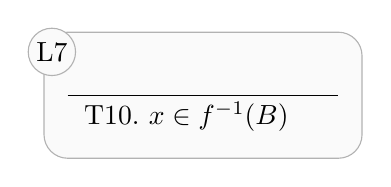
\begin{tikzpicture}[baseline=(main.base)]%
\node[tableau] (main) {%
\\

\begin{tabular}{ll}%

\Bstrut\\\hline\Tstrut
T10.\ $\textrm{$x\in f^{-1}(B)$}$&
\end{tabular}%
};%
\node[tableaulabel] at (main.north west) [xshift=4mm, yshift=-5.5mm] {L7};
\end{tikzpicture}%

\end{tabular}%
};%
\node[tableaulabel] at (main.north west) [xshift=4mm, yshift=-5.5mm] {L2};
\end{tikzpicture}%
\\
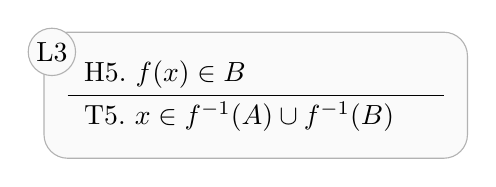
\begin{tikzpicture}[baseline=(main.base)]%
\node[tableau] (main) {%
\\

\begin{tabular}{ll}%
H5.\ $\textrm{$f(x)\in B$}$&
\Bstrut\\\hline\Tstrut
T5.\ $\textrm{$x\in f^{-1}(A)\cup f^{-1}(B)$}$&
\end{tabular}%
};%
\node[tableaulabel] at (main.north west) [xshift=4mm, yshift=-5.5mm] {L3};
\end{tikzpicture}%

\end{tabular}%
};%
\node[tableaulabel] at (main.north west) [xshift=4mm, yshift=-5.5mm] {L1};
\end{tikzpicture}%
\end{fit}
\smallskip

\noindent9. Hypothesis H4 matches target T11, so L6 is done.\nopagebreak[4] 
\marginpar{But this is clearly the case, so we are done.}\nopagebreak[4] 
\smallskip\nopagebreak[4] 

\begin{fit}\begin{tikzpicture}[baseline=(main.base)]%
\node[tableau] (main) {%
$x$\\

\begin{tabular}{ll}%

\Bstrut\\\hline\Tstrut
\begin{tikzpicture}[baseline=(main.base)]%
\node[tableau] (main) {%
\\

\begin{tabular}{ll}%
H4.\ $\textrm{$f(x)\in A$}$&
\Bstrut\\\hline\Tstrut
\begin{tikzpicture}%
\node[tableau] (main) {%
\ \ \,Done
};%
\node[tableaulabel] at (main.north west) [xshift=4mm, yshift=-5.5mm] {L6};
\end{tikzpicture}%
\hspace{2mm}$\vee$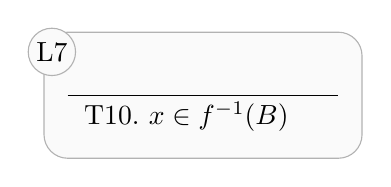
\begin{tikzpicture}[baseline=(main.base)]%
\node[tableau] (main) {%
\\

\begin{tabular}{ll}%

\Bstrut\\\hline\Tstrut
T10.\ $\textrm{$x\in f^{-1}(B)$}$&
\end{tabular}%
};%
\node[tableaulabel] at (main.north west) [xshift=4mm, yshift=-5.5mm] {L7};
\end{tikzpicture}%

\end{tabular}%
};%
\node[tableaulabel] at (main.north west) [xshift=4mm, yshift=-5.5mm] {L2};
\end{tikzpicture}%
\\
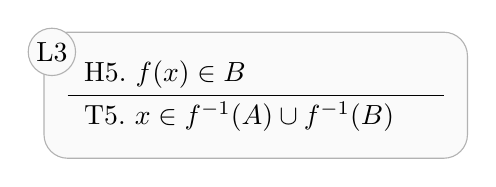
\begin{tikzpicture}[baseline=(main.base)]%
\node[tableau] (main) {%
\\

\begin{tabular}{ll}%
H5.\ $\textrm{$f(x)\in B$}$&
\Bstrut\\\hline\Tstrut
T5.\ $\textrm{$x\in f^{-1}(A)\cup f^{-1}(B)$}$&
\end{tabular}%
};%
\node[tableaulabel] at (main.north west) [xshift=4mm, yshift=-5.5mm] {L3};
\end{tikzpicture}%

\end{tabular}%
};%
\node[tableaulabel] at (main.north west) [xshift=4mm, yshift=-5.5mm] {L1};
\end{tikzpicture}%
\end{fit}
\smallskip

\noindent10. Some disjunct of the target of L2 is `Done', so L2 is itself `Done'.\nopagebreak[4] 
\marginpar{}\nopagebreak[4] 
\smallskip\nopagebreak[4] 

\begin{fit}\begin{tikzpicture}[baseline=(main.base)]%
\node[tableau] (main) {%
$x$\\

\begin{tabular}{ll}%

\Bstrut\\\hline\Tstrut
\begin{tikzpicture}%
\node[tableau] (main) {%
\ \ \,Done
};%
\node[tableaulabel] at (main.north west) [xshift=4mm, yshift=-5.5mm] {L2};
\end{tikzpicture}%
\\
\begin{tikzpicture}[baseline=(main.base)]%
\node[tableau] (main) {%
\\

\begin{tabular}{ll}%
H5.\ $\textrm{$f(x)\in B$}$&
\Bstrut\\\hline\Tstrut
T5.\ $\textrm{$x\in f^{-1}(A)\cup f^{-1}(B)$}$&
\end{tabular}%
};%
\node[tableaulabel] at (main.north west) [xshift=4mm, yshift=-5.5mm] {L3};
\end{tikzpicture}%

\end{tabular}%
};%
\node[tableaulabel] at (main.north west) [xshift=4mm, yshift=-5.5mm] {L1};
\end{tikzpicture}%
\end{fit}
\smallskip

\noindent11. Remove `Done' targets of L1.\nopagebreak[4] 
\marginpar{}\nopagebreak[4] 
\smallskip\nopagebreak[4] 

\begin{fit}\begin{tikzpicture}[baseline=(main.base)]%
\node[tableau] (main) {%
$x$\\

\begin{tabular}{ll}%

\Bstrut\\\hline\Tstrut
\begin{tikzpicture}[baseline=(main.base)]%
\node[tableau] (main) {%
\\

\begin{tabular}{ll}%
H5.\ $\textrm{$f(x)\in B$}$&
\Bstrut\\\hline\Tstrut
\textbf{\boldmath T5.\ $\textrm{$x\in f^{-1}(A)\cup f^{-1}(B)$}$\unboldmath }&\textbf{\boldmath \unboldmath }
\end{tabular}%
};%
\node[tableaulabel] at (main.north west) [xshift=4mm, yshift=-5.5mm] {L3};
\end{tikzpicture}%

\end{tabular}%
};%
\node[tableaulabel] at (main.north west) [xshift=4mm, yshift=-5.5mm] {L1};
\end{tikzpicture}%
\end{fit}
\smallskip

\noindent12. Quantifier-free expansion of target T5.\nopagebreak[4] 
\marginpar{We would like to show that $x\in f^{-1}(A)\cup f^{-1}(B)$, i.e. that $x\in f^{-1}(A)$ or $x\in f^{-1}(B)$.}\nopagebreak[4] 
\smallskip\nopagebreak[4] 

\begin{fit}\begin{tikzpicture}[baseline=(main.base)]%
\node[tableau] (main) {%
$x$\\

\begin{tabular}{ll}%

\Bstrut\\\hline\Tstrut
\begin{tikzpicture}[baseline=(main.base)]%
\node[tableau] (main) {%
\\

\begin{tabular}{ll}%
H5.\ $\textrm{$f(x)\in B$}$&
\Bstrut\\\hline\Tstrut
\textbf{\boldmath T12.\ $\textrm{$x\in f^{-1}(A)$}\vee \textrm{$x\in f^{-1}(B)$}$\unboldmath }&\textbf{\boldmath \unboldmath }
\end{tabular}%
};%
\node[tableaulabel] at (main.north west) [xshift=4mm, yshift=-5.5mm] {L3};
\end{tikzpicture}%

\end{tabular}%
};%
\node[tableaulabel] at (main.north west) [xshift=4mm, yshift=-5.5mm] {L1};
\end{tikzpicture}%
\end{fit}
\smallskip

\noindent13. Split up disjunctive target T12.\nopagebreak[4] 
\marginpar{}\nopagebreak[4] 
\smallskip\nopagebreak[4] 

\begin{fit}\begin{tikzpicture}[baseline=(main.base)]%
\node[tableau] (main) {%
$x$\\

\begin{tabular}{ll}%

\Bstrut\\\hline\Tstrut
\begin{tikzpicture}[baseline=(main.base)]%
\node[tableau] (main) {%
\\

\begin{tabular}{ll}%
H5.\ $\textrm{$f(x)\in B$}$&
\Bstrut\\\hline\Tstrut
\begin{tikzpicture}[baseline=(main.base)]%
\node[tableau] (main) {%
\\

\begin{tabular}{ll}%

\Bstrut\\\hline\Tstrut
\textbf{\boldmath T15.\ $\textrm{$x\in f^{-1}(A)$}$\unboldmath }&\textbf{\boldmath \unboldmath }
\end{tabular}%
};%
\node[tableaulabel] at (main.north west) [xshift=4mm, yshift=-5.5mm] {L10};
\end{tikzpicture}%
\hspace{2mm}$\vee$\begin{tikzpicture}[baseline=(main.base)]%
\node[tableau] (main) {%
\\

\begin{tabular}{ll}%

\Bstrut\\\hline\Tstrut
T16.\ $\textrm{$x\in f^{-1}(B)$}$&
\end{tabular}%
};%
\node[tableaulabel] at (main.north west) [xshift=4mm, yshift=-5.5mm] {L11};
\end{tikzpicture}%

\end{tabular}%
};%
\node[tableaulabel] at (main.north west) [xshift=4mm, yshift=-5.5mm] {L3};
\end{tikzpicture}%

\end{tabular}%
};%
\node[tableaulabel] at (main.north west) [xshift=4mm, yshift=-5.5mm] {L1};
\end{tikzpicture}%
\end{fit}
\smallskip

\noindent14. Quantifier-free expansion of target T15.\nopagebreak[4] 
\marginpar{We would like to show that $x\in f^{-1}(A)$, i.e. that $f(x)\in A$.}\nopagebreak[4] 
\smallskip\nopagebreak[4] 

\begin{fit}\begin{tikzpicture}[baseline=(main.base)]%
\node[tableau] (main) {%
$x$\\

\begin{tabular}{ll}%

\Bstrut\\\hline\Tstrut
\begin{tikzpicture}[baseline=(main.base)]%
\node[tableau] (main) {%
\\

\begin{tabular}{ll}%
H5.\ $\textrm{$f(x)\in B$}$&
\Bstrut\\\hline\Tstrut
\begin{tikzpicture}[baseline=(main.base)]%
\node[tableau] (main) {%
\\

\begin{tabular}{ll}%

\Bstrut\\\hline\Tstrut
T17.\ $\textrm{$f(x)\in A$}$&
\end{tabular}%
};%
\node[tableaulabel] at (main.north west) [xshift=4mm, yshift=-5.5mm] {L10};
\end{tikzpicture}%
\hspace{2mm}$\vee$\begin{tikzpicture}[baseline=(main.base)]%
\node[tableau] (main) {%
\\

\begin{tabular}{ll}%

\Bstrut\\\hline\Tstrut
\textbf{\boldmath T16.\ $\textrm{$x\in f^{-1}(B)$}$\unboldmath }&\textbf{\boldmath \unboldmath }
\end{tabular}%
};%
\node[tableaulabel] at (main.north west) [xshift=4mm, yshift=-5.5mm] {L11};
\end{tikzpicture}%

\end{tabular}%
};%
\node[tableaulabel] at (main.north west) [xshift=4mm, yshift=-5.5mm] {L3};
\end{tikzpicture}%

\end{tabular}%
};%
\node[tableaulabel] at (main.north west) [xshift=4mm, yshift=-5.5mm] {L1};
\end{tikzpicture}%
\end{fit}
\smallskip

\noindent15. Quantifier-free expansion of target T16.\nopagebreak[4] 
\marginpar{We would like to show that $x\in f^{-1}(B)$, i.e. that $f(x)\in B$.}\nopagebreak[4] 
\smallskip\nopagebreak[4] 

\begin{fit}\begin{tikzpicture}[baseline=(main.base)]%
\node[tableau] (main) {%
$x$\\

\begin{tabular}{ll}%

\Bstrut\\\hline\Tstrut
\begin{tikzpicture}[baseline=(main.base)]%
\node[tableau] (main) {%
\\

\begin{tabular}{ll}%
\textbf{\boldmath H5.\ $\textrm{$f(x)\in B$}$\unboldmath }&\textbf{\boldmath \unboldmath }
\Bstrut\\\hline\Tstrut
\begin{tikzpicture}[baseline=(main.base)]%
\node[tableau] (main) {%
\\

\begin{tabular}{ll}%

\Bstrut\\\hline\Tstrut
T17.\ $\textrm{$f(x)\in A$}$&
\end{tabular}%
};%
\node[tableaulabel] at (main.north west) [xshift=4mm, yshift=-5.5mm] {L10};
\end{tikzpicture}%
\hspace{2mm}$\vee$\begin{tikzpicture}[baseline=(main.base)]%
\node[tableau] (main) {%
\\

\begin{tabular}{ll}%

\Bstrut\\\hline\Tstrut
\textbf{\boldmath T18.\ $\textrm{$f(x)\in B$}$\unboldmath }&\textbf{\boldmath \unboldmath }
\end{tabular}%
};%
\node[tableaulabel] at (main.north west) [xshift=4mm, yshift=-5.5mm] {L11};
\end{tikzpicture}%

\end{tabular}%
};%
\node[tableaulabel] at (main.north west) [xshift=4mm, yshift=-5.5mm] {L3};
\end{tikzpicture}%

\end{tabular}%
};%
\node[tableaulabel] at (main.north west) [xshift=4mm, yshift=-5.5mm] {L1};
\end{tikzpicture}%
\end{fit}
\smallskip

\noindent16. Hypothesis H5 matches target T18, so L11 is done.\nopagebreak[4] 
\marginpar{But this is clearly the case, so we are done.}\nopagebreak[4] 
\smallskip\nopagebreak[4] 

\begin{fit}\begin{tikzpicture}[baseline=(main.base)]%
\node[tableau] (main) {%
$x$\\

\begin{tabular}{ll}%

\Bstrut\\\hline\Tstrut
\begin{tikzpicture}[baseline=(main.base)]%
\node[tableau] (main) {%
\\

\begin{tabular}{ll}%
H5.\ $\textrm{$f(x)\in B$}$&
\Bstrut\\\hline\Tstrut
\begin{tikzpicture}[baseline=(main.base)]%
\node[tableau] (main) {%
\\

\begin{tabular}{ll}%

\Bstrut\\\hline\Tstrut
T17.\ $\textrm{$f(x)\in A$}$&
\end{tabular}%
};%
\node[tableaulabel] at (main.north west) [xshift=4mm, yshift=-5.5mm] {L10};
\end{tikzpicture}%
\hspace{2mm}$\vee$\begin{tikzpicture}%
\node[tableau] (main) {%
\ \ \,Done
};%
\node[tableaulabel] at (main.north west) [xshift=4mm, yshift=-5.5mm] {L11};
\end{tikzpicture}%

\end{tabular}%
};%
\node[tableaulabel] at (main.north west) [xshift=4mm, yshift=-5.5mm] {L3};
\end{tikzpicture}%

\end{tabular}%
};%
\node[tableaulabel] at (main.north west) [xshift=4mm, yshift=-5.5mm] {L1};
\end{tikzpicture}%
\end{fit}
\smallskip

\noindent17. Some disjunct of the target of L3 is `Done', so L3 is itself `Done'.\nopagebreak[4] 
\marginpar{}\nopagebreak[4] 
\smallskip\nopagebreak[4] 

\begin{fit}\begin{tikzpicture}[baseline=(main.base)]%
\node[tableau] (main) {%
$x$\\

\begin{tabular}{ll}%

\Bstrut\\\hline\Tstrut
\begin{tikzpicture}%
\node[tableau] (main) {%
\ \ \,Done
};%
\node[tableaulabel] at (main.north west) [xshift=4mm, yshift=-5.5mm] {L3};
\end{tikzpicture}%

\end{tabular}%
};%
\node[tableaulabel] at (main.north west) [xshift=4mm, yshift=-5.5mm] {L1};
\end{tikzpicture}%
\end{fit}
\smallskip

\noindent18. All targets of L1 are `Done', so L1 is itself done.\nopagebreak[4] 
\marginpar{}\nopagebreak[4] 
\smallskip\nopagebreak[4] 

\begin{fit}\begin{tikzpicture}%
\node[tableau] (main) {%
\ \ \,Done
};%
\node[tableaulabel] at (main.north west) [xshift=4mm, yshift=-5.5mm] {L1};
\end{tikzpicture}%
\end{fit}

Problem solved.
\cleardoublepage

\end{steps}
{\begin{center} \large \textbf{Prove that $f^{-1}(A) \cup f^{-1}(B) \subset f^{-1}(A \cup B)$}\end{center}}\nopagebreak[4]

\begin{center}
\begin{minipage}{120mm}
Let $x$ be an element of $f^{-1}(A)\cup f^{-1}(B)$. Then $x\in f^{-1}(A)$ or $x\in f^{-1}(B)$. Since $x\in f^{-1}(A)$, we have that $f(x)\in A$. Since $x\in f^{-1}(B)$, we have that $f(x)\in B$. We would like to show that $x\in f^{-1}(A\cup B)$, i.e. that $f(x)\in A\cup B$. We would like to show that $f(x)\in A\cup B$, i.e. that $f(x)\in A$ or $f(x)\in B$. But this is clearly the case, so we are done. We would like to show that $x\in f^{-1}(A\cup B)$, i.e. that $f(x)\in A\cup B$. We would like to show that $f(x)\in A\cup B$, i.e. that $f(x)\in A$ or $f(x)\in B$. But this is clearly the case, so we are done.
\end{minipage}
\end{center}

\bigskip
\begin{steps}
\begin{fit}\begin{tikzpicture}[baseline=(main.base)]%
\node[tableau] (main) {%
\\

\begin{tabular}{ll}%

\Bstrut\\\hline\Tstrut
\textbf{\boldmath T1.\ $\textrm{$f^{-1}(A)\cup f^{-1}(B)\subset f^{-1}(A\cup B)$}$\unboldmath }&\textbf{\boldmath \unboldmath }
\end{tabular}%
};%
\node[tableaulabel] at (main.north west) [xshift=4mm, yshift=-5.5mm] {L1};
\end{tikzpicture}%
\end{fit}
\smallskip

\noindent1. Expand pre-universal target T1.\nopagebreak[4] 
\marginpar{}\nopagebreak[4] 
\smallskip\nopagebreak[4] 

\begin{fit}\begin{tikzpicture}[baseline=(main.base)]%
\node[tableau] (main) {%
\\

\begin{tabular}{ll}%

\Bstrut\\\hline\Tstrut
\textbf{\boldmath T2.\ $\forall x.(\textrm{$x\in f^{-1}(A)\cup f^{-1}(B)$}\Rightarrow \textrm{$x\in f^{-1}(A\cup B)$})$\unboldmath }&\textbf{\boldmath \unboldmath }
\end{tabular}%
};%
\node[tableaulabel] at (main.north west) [xshift=4mm, yshift=-5.5mm] {L1};
\end{tikzpicture}%
\end{fit}
\smallskip

\noindent2. Apply `let' trick and move premise of universal-conditional target T2 above the line.\nopagebreak[4] 
\marginpar{Let $x$ be an element of $f^{-1}(A)\cup f^{-1}(B)$.}\nopagebreak[4] 
\smallskip\nopagebreak[4] 

\begin{fit}\begin{tikzpicture}[baseline=(main.base)]%
\node[tableau] (main) {%
$x$\\

\begin{tabular}{ll}%
\textbf{\boldmath H1.\ $\textrm{$x\in f^{-1}(A)\cup f^{-1}(B)$}$\unboldmath }&\textbf{\boldmath \unboldmath }
\Bstrut\\\hline\Tstrut
T3.\ $\textrm{$x\in f^{-1}(A\cup B)$}$&
\end{tabular}%
};%
\node[tableaulabel] at (main.north west) [xshift=4mm, yshift=-5.5mm] {L1};
\end{tikzpicture}%
\end{fit}
\smallskip

\noindent3. Quantifier-free expansion of hypothesis H1.\nopagebreak[4] 
\marginpar{Since $x\in f^{-1}(A)\cup f^{-1}(B)$, $x\in f^{-1}(A)$ or $x\in f^{-1}(B)$.}\nopagebreak[4] 
\smallskip\nopagebreak[4] 

\begin{fit}\begin{tikzpicture}[baseline=(main.base)]%
\node[tableau] (main) {%
$x$\\

\begin{tabular}{ll}%
\textbf{\boldmath H2.\ $\textrm{$x\in f^{-1}(A)$}\vee \textrm{$x\in f^{-1}(B)$}$\unboldmath }&\textbf{\boldmath \unboldmath }
\Bstrut\\\hline\Tstrut
T3.\ $\textrm{$x\in f^{-1}(A\cup B)$}$&
\end{tabular}%
};%
\node[tableaulabel] at (main.north west) [xshift=4mm, yshift=-5.5mm] {L1};
\end{tikzpicture}%
\end{fit}
\smallskip

\noindent4. Split into cases to handle disjunctive hypothesis H2.\nopagebreak[4] 
\marginpar{}\nopagebreak[4] 
\smallskip\nopagebreak[4] 

\begin{fit}\begin{tikzpicture}[baseline=(main.base)]%
\node[tableau] (main) {%
$x$\\

\begin{tabular}{ll}%

\Bstrut\\\hline\Tstrut
\begin{tikzpicture}[baseline=(main.base)]%
\node[tableau] (main) {%
\\

\begin{tabular}{ll}%
\textbf{\boldmath H3.\ $\textrm{$x\in f^{-1}(A)$}$\unboldmath }&\textbf{\boldmath \unboldmath }
\Bstrut\\\hline\Tstrut
T4.\ $\textrm{$x\in f^{-1}(A\cup B)$}$&
\end{tabular}%
};%
\node[tableaulabel] at (main.north west) [xshift=4mm, yshift=-5.5mm] {L2};
\end{tikzpicture}%
\\
\begin{tikzpicture}[baseline=(main.base)]%
\node[tableau] (main) {%
\\

\begin{tabular}{ll}%
H4.\ $\textrm{$x\in f^{-1}(B)$}$&
\Bstrut\\\hline\Tstrut
T5.\ $\textrm{$x\in f^{-1}(A\cup B)$}$&
\end{tabular}%
};%
\node[tableaulabel] at (main.north west) [xshift=4mm, yshift=-5.5mm] {L3};
\end{tikzpicture}%

\end{tabular}%
};%
\node[tableaulabel] at (main.north west) [xshift=4mm, yshift=-5.5mm] {L1};
\end{tikzpicture}%
\end{fit}
\smallskip

\noindent5. Quantifier-free expansion of hypothesis H3.\nopagebreak[4] 
\marginpar{Since $x\in f^{-1}(A)$, we have that $f(x)\in A$.}\nopagebreak[4] 
\smallskip\nopagebreak[4] 

\begin{fit}\begin{tikzpicture}[baseline=(main.base)]%
\node[tableau] (main) {%
$x$\\

\begin{tabular}{ll}%

\Bstrut\\\hline\Tstrut
\begin{tikzpicture}[baseline=(main.base)]%
\node[tableau] (main) {%
\\

\begin{tabular}{ll}%
H5.\ $\textrm{$f(x)\in A$}$&
\Bstrut\\\hline\Tstrut
T4.\ $\textrm{$x\in f^{-1}(A\cup B)$}$&
\end{tabular}%
};%
\node[tableaulabel] at (main.north west) [xshift=4mm, yshift=-5.5mm] {L2};
\end{tikzpicture}%
\\
\begin{tikzpicture}[baseline=(main.base)]%
\node[tableau] (main) {%
\\

\begin{tabular}{ll}%
\textbf{\boldmath H4.\ $\textrm{$x\in f^{-1}(B)$}$\unboldmath }&\textbf{\boldmath \unboldmath }
\Bstrut\\\hline\Tstrut
T5.\ $\textrm{$x\in f^{-1}(A\cup B)$}$&
\end{tabular}%
};%
\node[tableaulabel] at (main.north west) [xshift=4mm, yshift=-5.5mm] {L3};
\end{tikzpicture}%

\end{tabular}%
};%
\node[tableaulabel] at (main.north west) [xshift=4mm, yshift=-5.5mm] {L1};
\end{tikzpicture}%
\end{fit}
\smallskip

\noindent6. Quantifier-free expansion of hypothesis H4.\nopagebreak[4] 
\marginpar{Since $x\in f^{-1}(B)$, we have that $f(x)\in B$.}\nopagebreak[4] 
\smallskip\nopagebreak[4] 

\begin{fit}\begin{tikzpicture}[baseline=(main.base)]%
\node[tableau] (main) {%
$x$\\

\begin{tabular}{ll}%

\Bstrut\\\hline\Tstrut
\begin{tikzpicture}[baseline=(main.base)]%
\node[tableau] (main) {%
\\

\begin{tabular}{ll}%
H5.\ $\textrm{$f(x)\in A$}$&
\Bstrut\\\hline\Tstrut
\textbf{\boldmath T4.\ $\textrm{$x\in f^{-1}(A\cup B)$}$\unboldmath }&\textbf{\boldmath \unboldmath }
\end{tabular}%
};%
\node[tableaulabel] at (main.north west) [xshift=4mm, yshift=-5.5mm] {L2};
\end{tikzpicture}%
\\
\begin{tikzpicture}[baseline=(main.base)]%
\node[tableau] (main) {%
\\

\begin{tabular}{ll}%
H6.\ $\textrm{$f(x)\in B$}$&
\Bstrut\\\hline\Tstrut
T5.\ $\textrm{$x\in f^{-1}(A\cup B)$}$&
\end{tabular}%
};%
\node[tableaulabel] at (main.north west) [xshift=4mm, yshift=-5.5mm] {L3};
\end{tikzpicture}%

\end{tabular}%
};%
\node[tableaulabel] at (main.north west) [xshift=4mm, yshift=-5.5mm] {L1};
\end{tikzpicture}%
\end{fit}
\smallskip

\noindent7. Quantifier-free expansion of target T4.\nopagebreak[4] 
\marginpar{We would like to show that $x\in f^{-1}(A\cup B)$, i.e. that $f(x)\in A\cup B$.}\nopagebreak[4] 
\smallskip\nopagebreak[4] 

\begin{fit}\begin{tikzpicture}[baseline=(main.base)]%
\node[tableau] (main) {%
$x$\\

\begin{tabular}{ll}%

\Bstrut\\\hline\Tstrut
\begin{tikzpicture}[baseline=(main.base)]%
\node[tableau] (main) {%
\\

\begin{tabular}{ll}%
H5.\ $\textrm{$f(x)\in A$}$&
\Bstrut\\\hline\Tstrut
\textbf{\boldmath T6.\ $\textrm{$f(x)\in A\cup B$}$\unboldmath }&\textbf{\boldmath \unboldmath }
\end{tabular}%
};%
\node[tableaulabel] at (main.north west) [xshift=4mm, yshift=-5.5mm] {L2};
\end{tikzpicture}%
\\
\begin{tikzpicture}[baseline=(main.base)]%
\node[tableau] (main) {%
\\

\begin{tabular}{ll}%
H6.\ $\textrm{$f(x)\in B$}$&
\Bstrut\\\hline\Tstrut
T5.\ $\textrm{$x\in f^{-1}(A\cup B)$}$&
\end{tabular}%
};%
\node[tableaulabel] at (main.north west) [xshift=4mm, yshift=-5.5mm] {L3};
\end{tikzpicture}%

\end{tabular}%
};%
\node[tableaulabel] at (main.north west) [xshift=4mm, yshift=-5.5mm] {L1};
\end{tikzpicture}%
\end{fit}
\smallskip

\noindent8. Quantifier-free expansion of target T6.\nopagebreak[4] 
\marginpar{We would like to show that $f(x)\in A\cup B$, i.e. that $f(x)\in A$ or $f(x)\in B$.}\nopagebreak[4] 
\smallskip\nopagebreak[4] 

\begin{fit}\begin{tikzpicture}[baseline=(main.base)]%
\node[tableau] (main) {%
$x$\\

\begin{tabular}{ll}%

\Bstrut\\\hline\Tstrut
\begin{tikzpicture}[baseline=(main.base)]%
\node[tableau] (main) {%
\\

\begin{tabular}{ll}%
H5.\ $\textrm{$f(x)\in A$}$&
\Bstrut\\\hline\Tstrut
\textbf{\boldmath T7.\ $\textrm{$f(x)\in A$}\vee \textrm{$f(x)\in B$}$\unboldmath }&\textbf{\boldmath \unboldmath }
\end{tabular}%
};%
\node[tableaulabel] at (main.north west) [xshift=4mm, yshift=-5.5mm] {L2};
\end{tikzpicture}%
\\
\begin{tikzpicture}[baseline=(main.base)]%
\node[tableau] (main) {%
\\

\begin{tabular}{ll}%
H6.\ $\textrm{$f(x)\in B$}$&
\Bstrut\\\hline\Tstrut
T5.\ $\textrm{$x\in f^{-1}(A\cup B)$}$&
\end{tabular}%
};%
\node[tableaulabel] at (main.north west) [xshift=4mm, yshift=-5.5mm] {L3};
\end{tikzpicture}%

\end{tabular}%
};%
\node[tableaulabel] at (main.north west) [xshift=4mm, yshift=-5.5mm] {L1};
\end{tikzpicture}%
\end{fit}
\smallskip

\noindent9. Split up disjunctive target T7.\nopagebreak[4] 
\marginpar{}\nopagebreak[4] 
\smallskip\nopagebreak[4] 

\begin{fit}\begin{tikzpicture}[baseline=(main.base)]%
\node[tableau] (main) {%
$x$\\

\begin{tabular}{ll}%

\Bstrut\\\hline\Tstrut
\begin{tikzpicture}[baseline=(main.base)]%
\node[tableau] (main) {%
\\

\begin{tabular}{ll}%
\textbf{\boldmath H5.\ $\textrm{$f(x)\in A$}$\unboldmath }&\textbf{\boldmath \unboldmath }
\Bstrut\\\hline\Tstrut
\begin{tikzpicture}[baseline=(main.base)]%
\node[tableau] (main) {%
\\

\begin{tabular}{ll}%

\Bstrut\\\hline\Tstrut
\textbf{\boldmath T10.\ $\textrm{$f(x)\in A$}$\unboldmath }&\textbf{\boldmath \unboldmath }
\end{tabular}%
};%
\node[tableaulabel] at (main.north west) [xshift=4mm, yshift=-5.5mm] {L6};
\end{tikzpicture}%
\hspace{2mm}$\vee$\begin{tikzpicture}[baseline=(main.base)]%
\node[tableau] (main) {%
\\

\begin{tabular}{ll}%

\Bstrut\\\hline\Tstrut
T11.\ $\textrm{$f(x)\in B$}$&
\end{tabular}%
};%
\node[tableaulabel] at (main.north west) [xshift=4mm, yshift=-5.5mm] {L7};
\end{tikzpicture}%

\end{tabular}%
};%
\node[tableaulabel] at (main.north west) [xshift=4mm, yshift=-5.5mm] {L2};
\end{tikzpicture}%
\\
\begin{tikzpicture}[baseline=(main.base)]%
\node[tableau] (main) {%
\\

\begin{tabular}{ll}%
H6.\ $\textrm{$f(x)\in B$}$&
\Bstrut\\\hline\Tstrut
T5.\ $\textrm{$x\in f^{-1}(A\cup B)$}$&
\end{tabular}%
};%
\node[tableaulabel] at (main.north west) [xshift=4mm, yshift=-5.5mm] {L3};
\end{tikzpicture}%

\end{tabular}%
};%
\node[tableaulabel] at (main.north west) [xshift=4mm, yshift=-5.5mm] {L1};
\end{tikzpicture}%
\end{fit}
\smallskip

\noindent10. Hypothesis H5 matches target T10, so L6 is done.\nopagebreak[4] 
\marginpar{But this is clearly the case, so we are done.}\nopagebreak[4] 
\smallskip\nopagebreak[4] 

\begin{fit}\begin{tikzpicture}[baseline=(main.base)]%
\node[tableau] (main) {%
$x$\\

\begin{tabular}{ll}%

\Bstrut\\\hline\Tstrut
\begin{tikzpicture}[baseline=(main.base)]%
\node[tableau] (main) {%
\\

\begin{tabular}{ll}%
H5.\ $\textrm{$f(x)\in A$}$&
\Bstrut\\\hline\Tstrut
\begin{tikzpicture}%
\node[tableau] (main) {%
\ \ \,Done
};%
\node[tableaulabel] at (main.north west) [xshift=4mm, yshift=-5.5mm] {L6};
\end{tikzpicture}%
\hspace{2mm}$\vee$\begin{tikzpicture}[baseline=(main.base)]%
\node[tableau] (main) {%
\\

\begin{tabular}{ll}%

\Bstrut\\\hline\Tstrut
T11.\ $\textrm{$f(x)\in B$}$&
\end{tabular}%
};%
\node[tableaulabel] at (main.north west) [xshift=4mm, yshift=-5.5mm] {L7};
\end{tikzpicture}%

\end{tabular}%
};%
\node[tableaulabel] at (main.north west) [xshift=4mm, yshift=-5.5mm] {L2};
\end{tikzpicture}%
\\
\begin{tikzpicture}[baseline=(main.base)]%
\node[tableau] (main) {%
\\

\begin{tabular}{ll}%
H6.\ $\textrm{$f(x)\in B$}$&
\Bstrut\\\hline\Tstrut
T5.\ $\textrm{$x\in f^{-1}(A\cup B)$}$&
\end{tabular}%
};%
\node[tableaulabel] at (main.north west) [xshift=4mm, yshift=-5.5mm] {L3};
\end{tikzpicture}%

\end{tabular}%
};%
\node[tableaulabel] at (main.north west) [xshift=4mm, yshift=-5.5mm] {L1};
\end{tikzpicture}%
\end{fit}
\smallskip

\noindent11. Some disjunct of the target of L2 is `Done', so L2 is itself `Done'.\nopagebreak[4] 
\marginpar{}\nopagebreak[4] 
\smallskip\nopagebreak[4] 

\begin{fit}\begin{tikzpicture}[baseline=(main.base)]%
\node[tableau] (main) {%
$x$\\

\begin{tabular}{ll}%

\Bstrut\\\hline\Tstrut
\begin{tikzpicture}%
\node[tableau] (main) {%
\ \ \,Done
};%
\node[tableaulabel] at (main.north west) [xshift=4mm, yshift=-5.5mm] {L2};
\end{tikzpicture}%
\\
\begin{tikzpicture}[baseline=(main.base)]%
\node[tableau] (main) {%
\\

\begin{tabular}{ll}%
H6.\ $\textrm{$f(x)\in B$}$&
\Bstrut\\\hline\Tstrut
T5.\ $\textrm{$x\in f^{-1}(A\cup B)$}$&
\end{tabular}%
};%
\node[tableaulabel] at (main.north west) [xshift=4mm, yshift=-5.5mm] {L3};
\end{tikzpicture}%

\end{tabular}%
};%
\node[tableaulabel] at (main.north west) [xshift=4mm, yshift=-5.5mm] {L1};
\end{tikzpicture}%
\end{fit}
\smallskip

\noindent12. Remove `Done' targets of L1.\nopagebreak[4] 
\marginpar{}\nopagebreak[4] 
\smallskip\nopagebreak[4] 

\begin{fit}\begin{tikzpicture}[baseline=(main.base)]%
\node[tableau] (main) {%
$x$\\

\begin{tabular}{ll}%

\Bstrut\\\hline\Tstrut
\begin{tikzpicture}[baseline=(main.base)]%
\node[tableau] (main) {%
\\

\begin{tabular}{ll}%
H6.\ $\textrm{$f(x)\in B$}$&
\Bstrut\\\hline\Tstrut
\textbf{\boldmath T5.\ $\textrm{$x\in f^{-1}(A\cup B)$}$\unboldmath }&\textbf{\boldmath \unboldmath }
\end{tabular}%
};%
\node[tableaulabel] at (main.north west) [xshift=4mm, yshift=-5.5mm] {L3};
\end{tikzpicture}%

\end{tabular}%
};%
\node[tableaulabel] at (main.north west) [xshift=4mm, yshift=-5.5mm] {L1};
\end{tikzpicture}%
\end{fit}
\smallskip

\noindent13. Quantifier-free expansion of target T5.\nopagebreak[4] 
\marginpar{We would like to show that $x\in f^{-1}(A\cup B)$, i.e. that $f(x)\in A\cup B$.}\nopagebreak[4] 
\smallskip\nopagebreak[4] 

\begin{fit}\begin{tikzpicture}[baseline=(main.base)]%
\node[tableau] (main) {%
$x$\\

\begin{tabular}{ll}%

\Bstrut\\\hline\Tstrut
\begin{tikzpicture}[baseline=(main.base)]%
\node[tableau] (main) {%
\\

\begin{tabular}{ll}%
H6.\ $\textrm{$f(x)\in B$}$&
\Bstrut\\\hline\Tstrut
\textbf{\boldmath T12.\ $\textrm{$f(x)\in A\cup B$}$\unboldmath }&\textbf{\boldmath \unboldmath }
\end{tabular}%
};%
\node[tableaulabel] at (main.north west) [xshift=4mm, yshift=-5.5mm] {L3};
\end{tikzpicture}%

\end{tabular}%
};%
\node[tableaulabel] at (main.north west) [xshift=4mm, yshift=-5.5mm] {L1};
\end{tikzpicture}%
\end{fit}
\smallskip

\noindent14. Quantifier-free expansion of target T12.\nopagebreak[4] 
\marginpar{We would like to show that $f(x)\in A\cup B$, i.e. that $f(x)\in A$ or $f(x)\in B$.}\nopagebreak[4] 
\smallskip\nopagebreak[4] 

\begin{fit}\begin{tikzpicture}[baseline=(main.base)]%
\node[tableau] (main) {%
$x$\\

\begin{tabular}{ll}%

\Bstrut\\\hline\Tstrut
\begin{tikzpicture}[baseline=(main.base)]%
\node[tableau] (main) {%
\\

\begin{tabular}{ll}%
H6.\ $\textrm{$f(x)\in B$}$&
\Bstrut\\\hline\Tstrut
\textbf{\boldmath T13.\ $\textrm{$f(x)\in A$}\vee \textrm{$f(x)\in B$}$\unboldmath }&\textbf{\boldmath \unboldmath }
\end{tabular}%
};%
\node[tableaulabel] at (main.north west) [xshift=4mm, yshift=-5.5mm] {L3};
\end{tikzpicture}%

\end{tabular}%
};%
\node[tableaulabel] at (main.north west) [xshift=4mm, yshift=-5.5mm] {L1};
\end{tikzpicture}%
\end{fit}
\smallskip

\noindent15. Split up disjunctive target T13.\nopagebreak[4] 
\marginpar{}\nopagebreak[4] 
\smallskip\nopagebreak[4] 

\begin{fit}\begin{tikzpicture}[baseline=(main.base)]%
\node[tableau] (main) {%
$x$\\

\begin{tabular}{ll}%

\Bstrut\\\hline\Tstrut
\begin{tikzpicture}[baseline=(main.base)]%
\node[tableau] (main) {%
\\

\begin{tabular}{ll}%
\textbf{\boldmath H6.\ $\textrm{$f(x)\in B$}$\unboldmath }&\textbf{\boldmath \unboldmath }
\Bstrut\\\hline\Tstrut
\begin{tikzpicture}[baseline=(main.base)]%
\node[tableau] (main) {%
\\

\begin{tabular}{ll}%

\Bstrut\\\hline\Tstrut
T16.\ $\textrm{$f(x)\in A$}$&
\end{tabular}%
};%
\node[tableaulabel] at (main.north west) [xshift=4mm, yshift=-5.5mm] {L10};
\end{tikzpicture}%
\hspace{2mm}$\vee$\begin{tikzpicture}[baseline=(main.base)]%
\node[tableau] (main) {%
\\

\begin{tabular}{ll}%

\Bstrut\\\hline\Tstrut
\textbf{\boldmath T17.\ $\textrm{$f(x)\in B$}$\unboldmath }&\textbf{\boldmath \unboldmath }
\end{tabular}%
};%
\node[tableaulabel] at (main.north west) [xshift=4mm, yshift=-5.5mm] {L11};
\end{tikzpicture}%

\end{tabular}%
};%
\node[tableaulabel] at (main.north west) [xshift=4mm, yshift=-5.5mm] {L3};
\end{tikzpicture}%

\end{tabular}%
};%
\node[tableaulabel] at (main.north west) [xshift=4mm, yshift=-5.5mm] {L1};
\end{tikzpicture}%
\end{fit}
\smallskip

\noindent16. Hypothesis H6 matches target T17, so L11 is done.\nopagebreak[4] 
\marginpar{But this is clearly the case, so we are done.}\nopagebreak[4] 
\smallskip\nopagebreak[4] 

\begin{fit}\begin{tikzpicture}[baseline=(main.base)]%
\node[tableau] (main) {%
$x$\\

\begin{tabular}{ll}%

\Bstrut\\\hline\Tstrut
\begin{tikzpicture}[baseline=(main.base)]%
\node[tableau] (main) {%
\\

\begin{tabular}{ll}%
H6.\ $\textrm{$f(x)\in B$}$&
\Bstrut\\\hline\Tstrut
\begin{tikzpicture}[baseline=(main.base)]%
\node[tableau] (main) {%
\\

\begin{tabular}{ll}%

\Bstrut\\\hline\Tstrut
T16.\ $\textrm{$f(x)\in A$}$&
\end{tabular}%
};%
\node[tableaulabel] at (main.north west) [xshift=4mm, yshift=-5.5mm] {L10};
\end{tikzpicture}%
\hspace{2mm}$\vee$\begin{tikzpicture}%
\node[tableau] (main) {%
\ \ \,Done
};%
\node[tableaulabel] at (main.north west) [xshift=4mm, yshift=-5.5mm] {L11};
\end{tikzpicture}%

\end{tabular}%
};%
\node[tableaulabel] at (main.north west) [xshift=4mm, yshift=-5.5mm] {L3};
\end{tikzpicture}%

\end{tabular}%
};%
\node[tableaulabel] at (main.north west) [xshift=4mm, yshift=-5.5mm] {L1};
\end{tikzpicture}%
\end{fit}
\smallskip

\noindent17. Some disjunct of the target of L3 is `Done', so L3 is itself `Done'.\nopagebreak[4] 
\marginpar{}\nopagebreak[4] 
\smallskip\nopagebreak[4] 

\begin{fit}\begin{tikzpicture}[baseline=(main.base)]%
\node[tableau] (main) {%
$x$\\

\begin{tabular}{ll}%

\Bstrut\\\hline\Tstrut
\begin{tikzpicture}%
\node[tableau] (main) {%
\ \ \,Done
};%
\node[tableaulabel] at (main.north west) [xshift=4mm, yshift=-5.5mm] {L3};
\end{tikzpicture}%

\end{tabular}%
};%
\node[tableaulabel] at (main.north west) [xshift=4mm, yshift=-5.5mm] {L1};
\end{tikzpicture}%
\end{fit}
\smallskip

\noindent18. All targets of L1 are `Done', so L1 is itself done.\nopagebreak[4] 
\marginpar{}\nopagebreak[4] 
\smallskip\nopagebreak[4] 

\begin{fit}\begin{tikzpicture}%
\node[tableau] (main) {%
\ \ \,Done
};%
\node[tableaulabel] at (main.north west) [xshift=4mm, yshift=-5.5mm] {L1};
\end{tikzpicture}%
\end{fit}

Problem solved.
\cleardoublepage

\end{steps}

\end{document}
